\documentclass[11pt,a4paper]{scrartcl}

% ------------------------------------------------------------

% Packages
\usepackage{mathtools}
\usepackage{amssymb}
\usepackage{tikz-qtree}
\usepackage[hidelinks]{hyperref}
\usepackage{caption}
\usepackage{titlesec}
\usepackage{tocloft}
\usepackage[cm]{fullpage}
\usepackage{csquotes}
\usepackage{wrapfig}
\usepackage{listings}
\usepackage{xcolor}
\usepackage{makeidx}
\usepackage{ulem}

\usepackage{graphicx}
\graphicspath{{images/}}

\usepackage{parskip}
\setlength{\parindent}{0pt}

%% Packages used for symbols and signs like (c), €
\usepackage{textcomp,units}
\usepackage{enumerate}

%% Package used for nice block text
\usepackage{microtype}

\usepackage{ellipsis}
\usepackage{fixltx2e}
\usepackage{booktabs}

%% Package used for correction of wrong display 'Marginalien'
\usepackage{mparhack}

%% Package used for nicer tables
\usepackage{longtable}

%% Packages used to break long urls
\usepackage{url}
\usepackage{etoolbox}
\appto\UrlBreaks{\do\a\do\b\do\c\do\d\do\e\do\f\do\g\do\h\do\i\do\j
\do\k\do\l\do\m\do\n\do\o\do\p\do\q\do\r\do\s\do\t\do\u\do\v\do\w
\do\x\do\y\do\z}

%% Package used for German descriptions
\usepackage[ansinew]{inputenc}
\usepackage[ngerman]{babel}
\addto\captionsngerman{ 
    \renewcommand{\figurename}{Abb.} 
    \renewcommand{\tablename}{Tabelle}
    \renewcommand{\abstractname}{Kurzfassung}
    %\renewcommand{\nomname}{Abkürzungen}
    \renewcommand{\lstlistingname}{Snippet}
    \renewcommand{\lstlistlistingname}{Verzeichnis der Snippets}
    \renewcommand{\indexname}{Stichwortverzeichnis}
}

\usepackage[automark]{scrpage2}
\automark[chapter]{chapter}
\clearscrheadfoot

% ------------------------------------------------------------

\newcommand{\AutorDominik} {
    \vspace{-4mm}
    \large \textbf{Autor:} Dominik Scharnagl \normalsize
    \vspace{2mm}
}


\newcommand{\AutorDominikFlorian} {
    \vspace{-4mm}
    \large \textbf{Autoren:} Dominik Scharnagl, Florian Boemmel \normalsize
    \vspace{2mm}
}

\newcommand{\AutorFlorian} {
    \vspace{-4mm}
    \large \textbf{Autor:} Florian Boemmel \normalsize
    \vspace{2mm}
}

\newcommand{\AutorFlorianNgoc} {
    \vspace{-4mm}
    \large \textbf{Autoren:} Florian Boemmel, Ngoc Luu Tran \normalsize
    \vspace{2mm}
}

\newcommand{\AutorNgoc} {
    \vspace{-4mm}
    \large \textbf{Autor:} Ngoc Luu Tran \normalsize
    \vspace{2mm}
}

\newcommand{\paratitle}[1] {
    \vspace{5mm}
    \large \textbf{#1} \normalsize
    \vspace{2mm}\newline
}

\newcommand{\paratitlecode}[2] {
    \vspace{5mm}
    \large \textbf{#1} \normalsize(\textit{\${#2}})
    \vspace{2mm}\newline
}

% Document Settings
%% Metadata
\title{\vspace{5cm}\huge Computer Architektur \\ \Large Studienarbeit \vspace{1cm}}
\subtitle{\Huge Emulation des Soundsystems \\ \Large Game Boy Advance Reverse Engineering \vspace{1cm}}
\author{\large \textbf{Dominik Scharnagl - Florian Boemmel - Ngoc Luu Tran}\\ \normalsize bei Nils Weis / Prof. Dr. Hackenberg}
\date{\normalsize 16. Mai 2018}

%% Language
%\selectlanguage{ngerman}

%% Colors
\definecolor{numberscolor}{RGB}{43,145,175}
\definecolor{commentcolor}{RGB}{0,128,0}
\definecolor{keywordcolor}{RGB}{0,0,255}

%% Formats
\titleformat*{\section}{\sffamily\huge\mdseries}
\titleformat*{\subsection}{\sffamily\LARGE\mdseries}
\titleformat*{\subsubsection}{\sffamily\Large\mdseries}

\def\trademark{\textsuperscript{\texttrademark}}

\lstset
{
    frame=single,
    captionpos=b,
    keepspaces=true,
    tabsize=4,
    showstringspaces=false,
    numbers=left, % display line numbers on the left
    basicstyle=\footnotesize\ttfamily,
    numberstyle=\color{numberscolor},
    commentstyle=\color{commentcolor},
    keywordstyle=\color{keywordcolor}
}

% ------------------------------------------------------------

% Commands
\renewcommand\cfttoctitlefont{\sffamily\hfill\Huge\mdseries}
\renewcommand\cftaftertoctitle{\sffamily\hfill\Large\mdseries\mbox{}}

\renewcommand{\cftsecfont}{\sffamily\Large\mdseries}
\renewcommand{\cftsubsecfont}{\sffamily\normalsize\mdseries}
\renewcommand{\cftsubsubsecfont}{\sffamily\normalsize\mdseries}

\renewcommand{\cftsecpagefont}{\sffamily\Large\mdseries}
\renewcommand{\cftsubsecpagefont}{\sffamily\normalsize\mdseries}
\renewcommand{\cftsubsubsecpagefont}{\sffamily\normalsize\mdseries}

%% Space between rows in tables
\renewcommand{\arraystretch}{1.5}

\makeindex

% ------------------------------------------------------------

\begin{document}
\sffamily

% ========== Title Page ==========
\maketitle
\thispagestyle{empty}

\vspace{5cm}
\begin{table}[h]
    \centering
    \begin{tabular}{ p{4cm} p{5cm}|p{5cm} p{2cm} }
        & \textbf{Autor} & \textbf{Matrikelnummer} & \\
        \hline
        & Dominik Scharnagl & 30 54 54 1 & \\
        & Florian Boemmel & 00 00 00 0 & \\
        & Ngoc Luu Tran & 30 32 96 3 &
    \end{tabular}
\end{table}


\clearpage

\setcounter{page}{1}

% ========== Table of Contents Page ==========

\pagenumbering{Roman}
\tableofcontents
\clearpage
\pagenumbering{arabic}

% ========== Index Page ==========

\printindex
\clearpage

% ========== Chapter 1 ==========

\section{Einleitung} \label{Einleitung}
\AutorFlorian

Der Game Boy Advance z\"ahlt zu einer der erfolgreichsten Spielekonsolen der Welt. Der 2001 von Nintendo \cite{NintendoGeschichte} ver\"offentlichte Nachfolger des Game Boy Classic findet sich heute noch in den Schubl\"aden der damalilgen Jugend. Deshalb \"uberrascht es auch nicht, dass die Fans der Konsole den Erinnerungen aus ihrer Kindheit neues Leben einhauchen und sogar Emulatoren f\"ur diverse Spiele-Klassiker der Plattform entwickeln.

\begin{figure}[h]
    \centering
    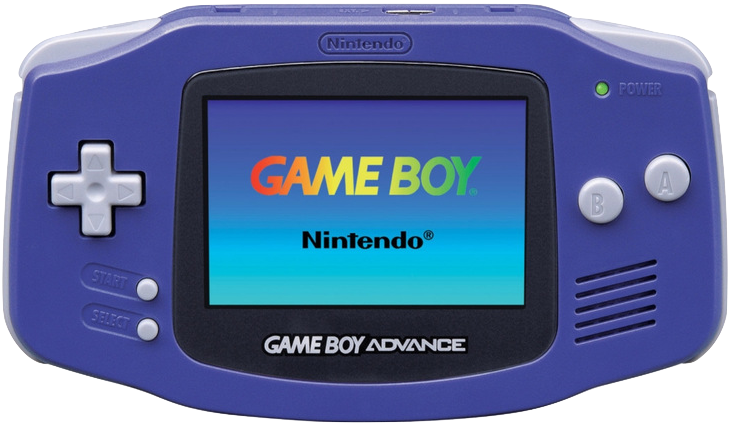
\includegraphics[width=0.5\textwidth]{GameBoyAdvance}
    \caption{Game Boy Advance - Blue Edition}
    \label{fig:gba}
\end{figure}

Der zentrale Inhalt der Studienarbeit, ist das Reverse Engineering eines solchen Game Boy Advance Emulators. Der genaue Inhalt dieser wird in den n\"achsten Kapiteln zun\"achst eingeschr\"ankt und sp\"ater weiter konkretisiert.

Emulatoren geh\"oren zu einem beliebten Werkzeug der Informatik. Sie bilden ein System oder ein Teilsystem ab. Dabei ist zu beachten, dass diese bekanntes Verhalten nur \enquote{nachahmen}. Genauer ausgef\"uhrt bedeutet dies, dass zum Beispiel bei einem Game Boy Advance Emulator die Software intern anders als auf dem originalen Ger\"at arbeitet. Jedoch kommt es beim Emulieren nicht auf die gleiche Arbeitsweise an, sondern auf das Ergebnis. In diesem konkreten Fall, einen voll funktionsf\"ahigen Nachbau des Game Boys in Software. Mit dem es m\"oglich ist digitalisierte Versionen eines Spieles spielen zu k\"onnen.\newline

\begin{table}[h]
    \centering
    \begin{tabular}{ r | p{10cm} }
        \textbf{CPU} & 16,77 MHz 32 Bit RISC (ARM7TDMI)\newline
              8 Bit CISC CPU (Z80/8080-Derivat) \\
        \hline
        \textbf{Arbeitsspeicher} & 32 KB IRAM (1 cycle/32 bit)\newline
                          + 96 KB VRAM (1-2 cycles)\newline
                          + 256 KB ERAM (6 cycles/32 bit) \\
        \hline
        \textbf{Lautsprecher} & Lautsprecher (Mono), Kopfh\"orer (Stereo) \\
    \end{tabular}
    \caption{Technische Daten des Game Boy Advance \cite{GameBoyTechnischeDaten}}
    \label{table:TechnischeDaten}
\end{table}

\newpage

\subsection{Untersuchungsgegenstand}
\AutorFlorian

In dieser Studienarbeit wird die Fragestellung, wie wird das Soundsystem des Game Boy Advance in einem beliebigen Emulator emuliert, thematisiert. Ein konkreter Emulator wurde nicht vorgegeben. Wir einigten uns demnach auf den Game Boy Advance Emulator \enquote{mGBA}. Dieser stellt im Folgenden unseren zentralen Untersuchungsgegenstand dar.

Die Untersuchung wird in vier Unterthemen gegliedert:

\begin{itemize}
    \item Erstellung eines Beispielprogramms (siehe Abschnitt \ref{Plattformen} und Abschnitt \ref{Softwareentwicklung})
    \item Untersuchung der Fragestellung mit Hilfe eines Beispielprogrammes (siehe Abschnitt \ref{Assemblercode})
    \item Untersuchung der Interaktion des Beispielprogrammes mit dem Emulator (siehe Abschnitt \ref{EmulationGameBoyAdvance})
    \item Untersuchung der Interaktion von Emulator und Betriebssystem (siehe Abschnitt \ref{EmulationSoundsystem})
\end{itemize}

\subsection{Verwendete Software}
\AutorFlorian

\begin{itemize}
    \item \textbf{Betriebssysteme}: Ubuntu 16.0 x64, Windows 10 x64, macOS 10.13.4
    \item \textbf{Disassembler}: IDA Pro, Sappy
    \item \textbf{Emualtor}: mGBA
    \item \textbf{SDK}: devkitPro
    \item \textbf{IDE's}: Programmer's Notepad, Visual Studio Code, Eclipse, Qt Creator
\end{itemize}

\newpage

% ========== Chapter 2 ==========

\section{Game Boy Advance} \label{GameBoyAdvance}
\AutorFlorianNgoc

\subsection{Hardwareumgebung} \label{Hardwareumgebung}
\AutorFlorian

Der Game Boy Advance verf\"ugt \"uber sechs Soundkan\"ale. Vier davon wurden, vor allem aus Gr\"unden der Abw\"artskompatibilit\"at, aus dem Vorg\"anger \enquote{Game Boy Classic} \"ubernommen.

\begin{table}[h]
    \centering
    \begin{tabular}{ r | p{10cm} }
        \textbf{Kanal} & \textbf{Art} \\
        \hline
        1 & Rechteckwellengenerator (square wave generator) \\
        \hline
        2 & Rechteckwellengenerator (square wave generator) \\
        \hline
        3 & Klangerzeuger (Sample-Player) \\
        \hline
        4 & Rauschgenerator (Noise-Generator) \\
        \hline
        A & Direct Sound \\
        \hline
        B & Direct Sound \\
    \end{tabular}
    \caption{\"Ubersicht der Soundkan\"ale des Game Boy Advance}
    \label{table:TechnischeDaten}
\end{table}

% ========== Chapter 2.1.1 ==========

\subsubsection{\"Ubersicht der Audio Register}
\AutorFlorian

Intern besitzt der Game Boy Advance drei Sound-Master-Register. Dort m\"ussen, je nach Einstellungswunsch, ein paar Bits gesetzt werden. Erst dann ist eine Soundwiedergabe oder die generelle Funktionsf\"ahigkeit des Soundsystems m\"oglich. \cite{GameBoySoundsystem}

Der Offset im Folgenden bezieht sich auf die Basisadresse $0x04000000$ und wird in hexadezimaler Schreibweise angegeben. An dieser Stelle muss darauf hingewiesen werden, dass die Bezeichnungen der Register nicht eindeutig sind und sich je nach verwendeter Quelle unterscheiden.

\begin{table}[h]
    \centering
    \begin{tabular}{ c | c | p{10cm} | l }
        \textbf{Offset} & \textbf{Kanal} & \textbf{Funktion} & \textbf{Bezeichnung} \\
        \hline
        $0x060$ & 1 & DMG Sweep control & \verb|SOUND1CNT_L| \\
        \hline
        $0x062$ & 1 & DMG Length, wave and evelope control & \verb|SOUND1CNT_H| \\
        \hline
        $0x064$ & 1 & DMG Frequency, reset and loop control & \verb|SOUND1CNT_X| \\
        \hline
        $0x068$ & 2 & DMG Length, wave and evelope control & \verb|SOUND2CNT_L| \\
        \hline
        $0x06C$ & 2 & DMG Frequency, reset and loop control & \verb|SOUND2CNT_H| \\
    \end{tabular}
    \caption{\"Ubersicht der Sound-Register - Teil 1}
    \label{table:SoundRegister1}
\end{table}

\newpage

\begin{table}[h]
    \centering
    \begin{tabular}{ c | c | p{10cm} | l }    
        \textbf{Offset} & \textbf{Kanal} & \textbf{Funktion} & \textbf{Bezeichnung} \\
        \hline
        $0x070$ & 3 & DMG Enable and wave ram bank control & \verb|SOUND3CNT_L| \\
        \hline
        $0x072$ & 3 & DMG Sound length and output level control & \verb|SOUND3CNT_H| \\
        \hline
        $0x074$ & 4 & DMG Frequency, reset and loop control & \verb|SOUND3CNT_X| \\
        \hline
        $0x078$ & 4 & DMG Length, output level and evelope control & \verb|SOUND4CNT_L| \\
        \hline
        $0x07C$ & 4 & DMG Noise parameters, reset and loop control & \verb|SOUND4CNT_H| \\
        \hline
        $0x080$ & & DMG Master Control & \verb|SOUNDCNT_L| \\
        \hline
        $0x082$ & & Direct Sound Master Control & \verb|SOUNDCNT_H| \\
        \hline
        $0x084$ & & Master Sound Output Control / Status & \verb|SOUNDCNT_X| \\
        \hline
        $0x088$ & & Sound Bias & \verb|SOUNDBIAS| \\
        \hline
        $0x090$ & 3 & DMG Wave RAM Register & \verb|WAVE_RAM0_L| \\
        \hline
        $0x092$ & 3 & DMG Wave RAM Register & \verb|WAVE_RAM0_H| \\
        \hline
        $0x094$ & 3 & DMG Wave RAM Register & \verb|WAVE_RAM1_L| \\
        \hline
        $0x096$ & 3 & DMG Wave RAM Register & \verb|WAVE_RAM1_H| \\
        \hline
        $0x098$ & 3 & DMG Wave RAM Register & \verb|WAVE_RAM2_L| \\
        \hline
        $0x09A$ & 3 & DMG Wave RAM Register & \verb|WAVE_RAM2_H| \\
        \hline
        $0x09C$ & 3 & DMG Wave RAM Register & \verb|WAVE_RAM3_L| \\
        \hline
        $0x09E$ & 3 & DMG Wave RAM Register & \verb|WAVE_RAM3_H| \\
        \hline
        $0x0A0$ & A & Direct Sound FIFO & \verb|FIFO_A_L| \\
        \hline
        $0x0A2$ & A & Direct Sound FIFO & \verb|FIFO_A_H| \\
        \hline
        $0x0A4$ & B & Direct Sound FIFO & \verb|FIFO_B_L| \\
        \hline
        $0x0A6$ & B & Direct Sound FIFO & \verb|FIFO_B_H| \\
    \end{tabular}
    \caption{\"Ubersicht der Sound-Register - Teil 2}
    \label{table:SoundRegister2}
\end{table}

Die in Tabelle \ref{table:SoundRegister1} und in Tabelle \ref{table:SoundRegister2} gelisteten Register sind im mGBA als Felder der Enumeration \textit{GBAIORegisters} (\textit{\$/include/mgba/internal/gba/io.h}) gelistet und entsprechend ihrer Registeradressen belegt. Sie werden unter anderen zur Adressierung des emulierten Speichers verwendet. Als Quelle f\"ur die beiden Tabellen diente neben der \textit{io.h} auch die Webseite \url{http://belogic.com/gba/}, Stand Juni 2018.

\newpage

% ========== Chapter 2.1.2 ==========

\subsubsection{\"Ubersicht der Sound Master Register}
\AutorFlorian

Die Register DMG Master Control, Direct Sound Master Control und Master Sound Output Control / Status bilden die Sound Master Register.

\paratitle{DMG Master Control} \label{dmgmastercontrol}
Hier m\"ussen zun\"achst einige Bits gesetzt werden, bevor eine generelle Verwendung des Soundsystems m\"oglich ist.

\begin{table}[h]
	\centering
    \begin{tabular}{ c | c | p{10cm} | l } 
	    \textbf{Bit} & \textbf{Kanal} & \textbf{Funktion} & \textbf{Bezeichnung} \\
	    \hline
	    0 & 1-4 & Left Volume & \\
	    \hline
	    1 & 1-4 & Left Volume & \\
	    \hline
	    2 & 1-4 & Left Volume & \\
	    \hline
	    3 & & & \\
	    \hline
	    4 & 1-4 & Right Volume & \\
	    \hline
	    5 & 1-4 & Right Volume & \\
	    \hline
	    6 & 1-4 & Right Volume & \\
	    \hline
	    7 & & & \\
	    \hline
	    8 & 1 & Channel 1 Left & \verb|SDMG_LSQR1| \\
	    \hline
	    9 & 2 & Channel 2 Left & \verb|SDMG_LSQR2| \\
	    \hline
	    A & 3 & Channel 3 Left & \verb|SDMG_LWAVE| \\
	    \hline
	    B & 4 & Channel 4 Left & \verb|SDMG_LNOISE| \\
	    \hline
	    C & 1 & Channel 1 Right & \verb|SDMG_RSQR1| \\
	    \hline
	    D & 2 & Channel 2 Right & \verb|SDMG_RSQR2| \\
	    \hline
	    E & 3 & Channel 3 Right & \verb|SDMG_RWAVE| \\
	    \hline
	    F & 4 & Channel 4 Right & \verb|SDMG_RNOISE| \\
	\end{tabular}
	\caption{DMG Master Control Register}
	\label{table:DmgMasterControlRegister}
\end{table}

\newpage

\paratitle{Direct Sound Master Control} \label{directsoundmastercontrol}
Dieses Register kontrolliert die Lautst\"arke der DMG Kan\"ale und aktiviert diese. Die Einstellungen k\"onnen separiert voneinander f\"ur den linken und rechten Lautsprecher vorgenommen werden.

\begin{table}[h]
	\centering
    \begin{tabular}{ c | c | p{10cm} | l } 
	    \textbf{Bits} & \textbf{Name} & \textbf{Funktion} & \textbf{Bezeichnung} \\
	    \hline
	    0-1 & DMGV & DMG Volume Ratio & \\
	        &      & 00: 25\% & \verb|SDS_DMG25| \\
	        &      & 01: 50\% & \verb|SDS_DMG50| \\
	        &      & 10: 100\% & \verb|SDS_DMG100| \\
	        &      & 11: forbidden \\
	    \hline
	    2 & AV & Direct Sound A Volume Ratio & \\
	      &    & 50\% if clear & \verb|SDSA50| \\
	      &    & 100\% if set  & \verb|SDSA100| \\
        \hline
	    3 & BV & Direct Sound B Volume Ratio & \\
	      &    & 50\% if clear & \verb|SDSB50| \\
	      &    & 100\% if set  & \verb|SDSB100| \\
	    \hline
	    4-7 & & & \\
	    \hline
	    8 & AR & Direct Sound A enable Direct Sound on Right speaker & \verb|SDS_AR| \\
	    \hline
	    9 & AL & Direct Sound A enable Direct Sound on Left speaker & \verb|SDS_AL| \\
	    \hline
	    A & AT & Direct Sound A Timer. & \\
	       &   & Use timer 0 (if clear) for Direct Sound A & \verb|SDS_ATMR0| \\
	       &   & Use timer 1 (if set) for Direct Sound A & \verb|SDS_ATMR1| \\
	    \hline
	    B & AF & FIFO reset for Direct Sound A & \verb|SDS_ARESET| \\
	    \hline
	    C & BR & Direct Sound B enable Direct Sound on Right speaker & \verb|SDS_BR| \\
	    \hline
	    D & BL & Direct Sound B enable Direct Sound on Left speaker & \verb|SDS_BL| \\
	    \hline
	    E & BT & Direct Sound B Timer. & \\
	       &   & Use timer 0 (if clear) for Direct Sound B & \verb|SDS_BTMR0| \\
	       &   & Use timer 1 (if set) for Direct Sound B & \verb|SDS_BTMR1| \\
	    \hline
	    F & BF & FIFO reset for Direct Sound B & \verb|SDS_BRESET| \\
	\end{tabular}
	\caption{Direct Sound Master Control Register}
	\label{table:DirectSoundMasterControlRegister}
\end{table}

Wenn DMA f\"ur Direct Sound verwendet wird, dann wird DMA den FIFO-Puffer zur\"ucksetzen, nachdem er verwendet wurde.


\newpage	
\paratitle{Master Sound Output Control / Status} \label{mastersoundoutputcontrol}
Aus diesem Register kann zu einem der Status der einzelnen DMG Kan\"ale ausgelesen werden und zum Anderen die generelle Soundausgabe aktiviert werden. Dazu muss das Bit 7 gesetzt werden.

\begin{table}[h]
	\centering
    \begin{tabular}{ c | c | p{10cm} | l } 
	    \textbf{Bits} & \textbf{Name} & \textbf{Funktion} & \textbf{Bezeichnung} \\
	    \hline
	    0 & 1A & Channel 1 is active and currently playing. & \verb|SSTAT_SQR1| \\
	    \hline
	    1 & 2A & Channel 2 is active and currently playing. & \verb|SSTAT_SQR2| \\
	    \hline
	    2 & 3A & Channel 3 is active and currently playing. & \verb|SSTAT_WAVE| \\
	    \hline
	    3 & 4A & Channel 4 is active and currently playing. & \verb|SSTAT_NOISE| \\
	    \hline
	    4-6 & & & \\
	    \hline
	    7 & MSE & Master Sound Enable & \verb|SSTAT_DISABLE| \\
	      &     & Must be set if any sound is to be heard at all. Set this before you do anything; otherwise other sound registers can't be accessed (see GBATek for more details). & \verb|SSTAT_ENABLE| \\
	    \hline
	    8-F & & & \\
	\end{tabular}
	\caption{Master Sound Output / Status Register}
	\label{table:MasterSoundOutputControlStatusRegister}
\end{table}

Die Bits 0-3 geben ausschlie{\ss}lich dar\"uber Auskunft, welcher Kanal aktuelle bespielt wird und nicht ob dieser eingeschaltet ist. Zum Ein- und Ausschalten eines Kanals dient das DMG Master Control Register (siehe Abschnitt \ref{dmgmastercontrol}).


% ========== Chapter 2.2 ==========

\newpage
\subsection{Plattformen} \label{Plattformen}
\AutorNgoc

% ========== Chapter 2.2.1 ==========

\subsubsection{DevkitPro}
\AutorNgoc

DevkitPro ist eine Organisation welche sich auf Cross-Compiler f\"ur beliebte Videospielkonsolen spezialisiert hat.

Das Ziel dabei ist es Hobby und Amateur Videospielentwicklern eine Plattform zu bieten, in welcher sie wertvolle Erfahrungen im Programmieren f\"ur Ressourcen limitierte Ger\"ate sammeln k\"onnen. Im Idealfall k\"onnen sie die gesammelten Erfahrungen dann auf eine Karriere in der Videospielentwicklung \"ubertragen.

Angefangen hat alles im Jahre 2003 mit dem Cross-Compiler namens devkitARM, welcher es erm\"oglichte Spiele f\"ur den Gambe Boy Advance zu entwickeln. Mittlerweile umfasst das Angebot nicht nur den Gambe Boy Advance, sondern auch den Nintendo GameCube, Nintendo Wii, GP32, Nintendo DS, GP2X und die Nintendo Switch. 

DevkitARM ist dabei nicht nur die erste Toolchain f\"ur Videospielkonsolen, sondern sie ist bis dato auch die beliebteste unter den Toolchains. So kammen \"uber die Jahre immer weitere ARM basierende Konsolen hinzu und entwickelte sich somit allgemein zu einen der besten Windows basierenden Entwicklertools f\"ur ARM-Ger\"ate. 

% ========== Chapter 2.2.2 ==========

\subsubsection{Belogic}
\AutorNgoc
 
Belogic ist eine Webseite welche einen Audio Development f\"ur Game Boy Advance Spiele n\"aher bringt. Die Seite ist insofern Hilfreich, da einen nicht nur die ganzen Sound Register erkl\"art werden, sondern auch jeder der 6 Channels. Zus\"atzlich wird zu jedem der 6 Channels auch ein Beispiel ROM mit entsprechendem Sourcecode zu Verf\"ugung gestellt.

Im Sourcecode gibt es auch ein entsprechenden Header, bei welchem schon alle Register und Sound Channels vordefiniert sind.

\vspace{5mm}
\begin{lstlisting}[language=C++, caption={1. Ausschnitt aus Belogic gba.h}, label={list:gbaheader2}]
    ...
	#define SOUND1PLAYONCE		0x4000		// play sound once
	#define SOUND1PLAYLOOP		0x0000		// play sound looped
	#define SOUND1INIT			0x8000		// makes the sound restart
	#define SOUND1SWEEPSHIFTS(n)	n		// number of sweep shifts (0-7)
	#define SOUND1SWEEPINC		0x0000		// sweep add (freq increase)
	#define SOUND1SWEEPDEC		0x0008		// sweep dec (freq decrese)
	#define SOUND1SWEEPTIME(n)	(n<<4)		// time of sweep (0-7)
	#define SOUND1ENVSTEPS(n)	(n<<8)		// envelope steps (0-7)
	#define SOUND1ENVINC		0x0800		// envellope increase
	#define SOUND1ENVDEC		0x0000		// envellope decrease
	#define SOUND1ENVINIT(n)	(n<<12)		// initial envelope volume (0-15)
	...
\end{lstlisting}

So erleichtert es einem das Programmieren auf Dauer doch sehr Erheblich, wenn man anstelle von "`*(vu16*)0x4000064 = 0x8000"', um den Sound Neustarten zulassen, "`REG\_SOUND1CNT\_X = SOUND1INIT"' schreiben kann.
\newpage
\vspace{5mm}
\begin{lstlisting}[language=C++, caption={2. Ausschnitt aus Belogic gba.h}, label={list:gbaheader1}]
    ...
	#define REG_SOUND1CNT   *(vu32*)0x4000060	//sound 1
	#define REG_SOUND1CNT_L *(vu16*)0x4000060	//
	#define REG_SOUND1CNT_H *(vu16*)0x4000062	//
	#define REG_SOUND1CNT_X *(vu16*)0x4000064	//

	#define REG_SOUND2CNT_L *(vu16*)0x4000068	//sound 2 lenght & wave duty
	#define REG_SOUND2CNT_H *(vu16*)0x400006C	//sound 2 frequency+loop+reset
	...
\end{lstlisting}

% ========== Chapter 2.2.3 ==========

\subsubsection{\enquote{Sappy}}
\AutorNgoc

Die von Nintendo bereitgestellte Sound-Engine, welche von der Mehrheit der kommerziellen Game Boy Advance Spielen genutzt wird, wird in der Rom-Hacking-Szene Sappy genannt. 
Der Name der Engine stammt von einem Programm namens Sappy, welches Musik aus den Game Boy Advance Spielen extrahiert und diese in MIDI-Dateien konvertiert.


Videospielentwickler komponieren ihre Musik als Standard MIDI-Datei oder als Trackermodul und konvertieren diese dann mithilfe eines Programms in das \enquote{Sappy-Format}. Dieses Format ist sehr \"ahnlich zu der MIDI-Datei und besteht unter anderem aus Key-On, Key-Off und Delta-T Werten. Jedoch wird das Sappy-Format effizienter gespeichert und wurde speziell f\"ur Videospiele entwickelt um zus\"atzlich noch sowas wie Soundeffekte abzuspielen.

Die Daten werden normalerweise in folgender Reihenfolge auf dem GBA-ROM gespeichert:
\vspace{15pt}
\begin{itemize}
\item Definitionen der Instrument Banks
\begin{itemize}
\item Sampled Instrument, Programmable-Sound-Generator (PSG) Instrument
\end{itemize}
\item Key-split Instrument Daten
\begin{itemize}
\item Key Split, Every Key-Split
\end{itemize}
\item Gameboy Channel 3 Waveform Daten
\item Track-Group RAM Zeiger
\item Musik/SFX Zeiger
\item Samples
\item Daten f\"ur jeden Track
\item Zeiger auf jeden Track
\end{itemize}
\vspace{15pt}

Die Daten m\"ussen nicht Zwangsl\"aufig in dieser Reihenfolge in einer ROM gespeichert sein und es ist ebenso m\"oglich, dass andere Daten dazwischen verschachtelt sind.

\vspace{15pt}
\textbf{{\large Voice Tabelle}}

Eine Voice Tabelle ist eine Ansammlung Zeigern zu Instrumenten, welches der Song benutzten kann. Diese besteht f\"ur gew\"ohnlich aus 127 Instrumenten, obwohl manche davon ungenutzt sein k\"onnen. 

So beinhaltet dieser unter anderen Sampled Instrument, PSG Instrument, Sub-Instrument, Key-Split Instrumente und Every-Key-Split Instrumente.

\newpage
\paratitle{Definition der Generischen Instrumenten Daten}
Jede Definition von einem Instrument oder Sub-Instruments besteht aus 12 Bytes, dabei gibt das erste Byte an um welchen Typen von Instrument es sich handelt.

\begin{table}[h]
    \centering
    \begin{tabular}{ c | p{15cm} }
        \textbf{HEX-Zahl} & \textbf{Instrumenten-Typ} \\
        \hline
        0x00 & Sample (GBA Direct Sound channel) \\
        \hline
        0x01 & Rechteckwellengenerator (Game Boy channel 1) \\
        \hline
        0x02 & Rechteckwellengenerator (Game Boy channel 2) \\
        \hline
        0x03 & PSG Programmable Waveform (Game Boy channel 3) \\
        \hline
        0x04 & Rauschgenerator (Game Boy channel 4) \\
        \hline
        0x08 & Sample (GBA Direct Sound channel) that is never resampled (always playing at the engine's rate) \\
				\hline
        0x09-0x0C & selbige wie 0x01-0x04\\
				\hline
        0x40 & Key split instrument  : Points to different sub-instruments depending on MIDI key \\
				\hline
        0x80 & Every Key split instrument / percussion : Each MIDI key points to its own sub-instrument anything else = invalid (the engine crashes) \\
    \end{tabular}
    \caption{\"ubersicht des Instrumententypes}
    \label{table:InstrumentenTyp}
\end{table}

\paratitle{Sampled Instrument / Sub-Instrument Format}
Um ein Sampled Instrument unver\"andert, also ohne Anwendung von Attack, Decay, Sustain und Release abzuspielen, werden die Werte 0xFF, 0x00, 0xFF, 0x00 verwendet.

\begin{table}[h]
    \centering
    \begin{tabular}{ c | p{15cm} }
        \textbf{Byte-Gr\"o{\ss}e} & \textbf{Definition} \\
        \hline
				1 & 0x00 (normal) oder 0x08 (nicht resampled) \\
				\hline
        1 & MIDI key (only used as percussion sub-instrument) \\
				\hline
        1 & nicht genutzt (immer 0) \\
				\hline
        1 & panning (only used as percussion sub-instrument).
         If bit 7 is set, the lower 7 bits forces the panning value for this key. Otherwise, the channel's panning is used \\
				\hline
        4 & Pointer zu Sample Dateien \\
				\hline
				1 & Attack-Wert (8-bit : 0x01 = l\"angster Attack, 0xFF = kein Attack) \\
        \hline
        1 & Decay-Wert (8-bit : 0x00 = kein Decay, 0xFF = l\"angster Decay) \\ 
        \hline
				1 & Sustain-Level (8-bit : 0x00 = Sustain zu Stumm, 0xFF = Sustain zur vollen Lautstl\"arke) \\
        \hline
        1 & Release-Wert (8-bit : 0x00 = sofortiger Release, 0xFF = l\"angster Release) \\
    \end{tabular}
    \caption{Sampled Instrument / Sub-Instrument Format}
    \label{table:SampleInstrument}
\end{table}


\newpage
\paratitle{PSG Instrument / Sub-Instrument Format}
Um ein PSG Instrument unver\"andert, also ohne Anwendung von Attack, Decay, Sustain und Release abzuspielen, werden die Werte 0xFF, 0x00, 0xFF, 0x00 verwendet.

\begin{table}[h]
    \centering
    \begin{tabular}{ c | p{15cm} }
        \textbf{Byte-Gr\"o{\ss}e} & \textbf{Definition} \\
				\hline
				1 & PSG Channel (0x01 = square 1, 0x02 = square 2, 0x03 = Programmierbare Waveform, 0x04 = Noise) \\
				\hline
        1 & MIDI Key (wird nur als Percussion Sub-Instrument verwendet)\\
				\hline
        1 & Hardware Time length Control (0x00 um Time length zu deaktivieren)\\
				\hline
        1 & Sweep Control (nur Square 1 Channel, 0x08 um Sweep zu deaktivieren) \\
				\hline
        4 & Square Channel:\newline
					1 Byte = Duty Cycle (0=12,5\%, 1=25\%, 2=50\%, 3=75\%)\newline
					3 Bytes = 0x0000\newline		
					Noise Channel:\newline	
					1 Byte = Steuert Noise's Periode (0 = Normal (32767 Samples), 1 = Metallic (127 Samples)) \newline
					3 bytes = 0x0000
					\newline
					Programmierbarer Channel:\newline
                4 bytes = Zeiger auf 16-Byte Waveform-Datei \\
				\hline
        1 & Attack-Wert (8-bit : 0x01 = l\"angster Attack, 0xFF = kein Attack)\\
				\hline
        1 & Decay-Wert (8-bit : 0x00 = kein Decay, 0xFF = l\"angster Decay) \\
				\hline
        1 & Sustain-Level (8-bit : 0x00 = Sustain zu Stumm, 0xFF = Sustain zur vollen Lautstl\"arke) \\
				\hline
        1 & Release-Wert (8-bit : 0x00 = sofortiger Release, 0xFF = l\"angster Release) \\
				
    \end{tabular}
    \caption{PSG Instrument / Sub-instrument Format}
    \label{table:PSGInstrument}
\end{table}
\vspace{-5pt}

\paratitle{Square \& Noise Channels}
Da die H\"ullkurve durch das ansteigen bzw. verringern des Hardware Volume Registers bestimmt wird, unterscheidet die sich grunds\"atzlich von den  Software emulierten Attack, Decay, Sustain und Release des Sampled Instrument.

Ein Beispiel hierf\"ur w\"ahre wenn Volume auf 6 ist, wird ein Attack von \enquote{3} doppelt so schnell ausgef\"uhrt wie der Attack von \enquote{3} wenn Volume 12 ist. Dies geschieht, weil Volume unabh\"angig vom Volume Wert, in der gleichen Rate ansteigt.

Zus\"atzlich kommt zu diesem Problem hinzu, dass bei jeder \"anderung von Volume in den Tracks sich Attack, Decay, Sustain und Release zur\"ucksetzen. Dies wiederum setzt den Sound zur\"uck, welches in ein \enquote{klick} Sound resultiert. Das kann auch in Spiele, welche Musik Volume ein und aus blenden, geh\"ohrt werden. Aus diesem Grund sollten Volume-\"anderungen vermieden werden und stattdessen falls m\"oglich Attack, Decay, Sustain und Release verwendet werden.

\paratitle{Programmierbarer Waveform Channel}
Die H\"ullkurve wird mit den vier Level welche f\"ur Volume zuverf\"ugung steht (25\%, 50\%, 75\% and 100\%) von der Software simuliert. Deswegen kann die H\"ullkurve sehr abgehackt und grob klingen, da nur sowenig Level zuverf\"ugung stehen. Jedoch leidet dieser Channel nicht unter dem Problem des Klickens bei Volume-\"anderung, wie bei den Square \& Noise Channels.


\newpage
\paratitle{Key-Split/Every Key-Split Instrumente}

\begin{table}[h]
    \centering
    \begin{tabular}{ c | p{7,5cm} | p{7,5cm}}
        \textbf{Byte-Gr\"o{\ss}e} & \textbf{Key Split Definition} & \textbf{Every Key-Split Definition}\\
        \hline
        1 & 0x40 & 0x80\\
				\hline
        3 & 0x00 & 0x00\\
				\hline
        4 & Zeiger auf ersten Sub-Instrument & Zeiger auf Percussion Tabelle \\
				\hline
        4 & Zeiger auf Key Split Tabelle & 0x00\\
    \end{tabular}
    \caption{Key-Split/Every Key-Split Instrumente}
    \label{table:EveryKey-SplitInstrument}
\end{table}


\paratitle{Key-Split}
Die Key-Split Tabelle hat eine L\"ange von 128 Bytes und gibt Informationen dar\"uber welches Sub-Instrument bei welchem MIDI-Key (1 Byte) genutzt wird. 
Die Position des benutzten Sub-Instrumentes ist:\newline 12 * KeySplitTable[MidiKey] + Zeiger auf ersten Sub-Instrument

\paratitle{Every Key-Split}
Die Position des benutzten Sub-Instrumentes ist:\newline 12 * MidiKey + Zeiger auf Percussion Tabelle.\newline
Der MIDI-Key und das Panning des spezifizierten Instruments wird nur hier benutzt.


\paratitle{Ungenutztes Instrumente}
HEX-Folge von einem ungenutzten Instrument:

0x01, 0x3C, 0x00, 0x00, 0x02, 0x00, 0x00, 0x00, 0x00, 0x00, 0x0F, 0x00

Aus irgendeinem Grund werden nicht genutzte Instrumente in der Sappy Sound Engine immer gleich definiert. W\"urde diese mutwillig Abgespielt werden, w\"urde es sich um ein PSG Square 1 ohne richtig aktivierten Sweep handeln (tiefe Oktaven werden nciht abgespielt).
		
\paratitle{\large 16-Byte programmaierbare Waveform Format}
Die Waveform besteht aus 32 4-Bit Puls-Code-Modulation (PCM) Samples, Big Endian, Unsigned (0 = niedriges Level, F = H\"oheres Level) f\"ur Insgesamt 16-bytes pro Waveform.

Zum Beispiel:

0x01, 0x23, 0x45, 0x67, 0x89, 0xAB, 0xCD, 0xEF, 0xFE, 0xDC, 0xBA, 0x98, 0x76, 0x54, 0x32, 0x10

Die konstante Erh\"ohung bis 0xFE und dann konstanter Fall des Wertes,wird eine Triangle Wave produzieren.

Der Game Boy Advance besitzt auch ein 64 Sample-Modus, jedoch keine bekannte M\"oglichkeit diesen Modus auszul\"osen.

\newpage
\paratitle{Track-Gruppen RAM Zeiger Format}
Die Sappy Sound Engine kann mehrere \enquote{Gruppen von Tracks} gleichzeitig wiedergeben, so k\"onnen Sound-Effekte abgespielt werden w\"ahrend Hintergrundmusik l\"auft. Verschiedene Spiele handhaben die Gruppen auf verschiedene Wegen.

\begin{table}[h]
    \centering
    \begin{tabular}{ c | p{15cm} }
        \textbf{Byte-Gr\"o{\ss}e} & \textbf{Definition}\\
        \hline
        4 & Zeiger auf Track-Gruppen Variablen, besteht aus 0x40 Bytes\\
				\hline
        4 & Zeiger auf Track Variablen, jeder Track besteht aus 0x50 Bytes\\
				\hline
        1 & Maximale Anzahl von Tracks f\"ur diese Gruppe. Falls versucht wird ein Song mit mehr Tracks abzuspielen, werden die \"uberschrittenen Tracks ignoriert und nciht abgespielt\\
				\hline
        3 & 0x00, 0x00, 0x00\\
    \end{tabular}
    \caption{Track-Gruppen RAM Zeiger Format}
    \label{table:RAMZeiger}
\end{table}

Die Sappy Sound Engine kann mehrere "Gruppen von Tracks" gleichzeitig wiedergeben, so k\"onnen Sound-Effekte abgespielt werden w\"ahrend Hintergrundmusik l\"auft. Verschiedene Spiele handhaben die Gruppen auf verschiedene Wegen.

Allen Anschein nach wei{\ss} das Spiel beim Start eines Songs nicht in welcher Gruppe es Anf\"angt, dies wird von der Song Zeiger Struktur entschieden. Danach kann aber Volume, Panning und andere Einstellungen durch Referenzen zur Gruppe, in welcher die Songs spielen, ver\"andert werden.

Jeder Track in jeder Gruppe hat sein eigenen Satz an Zeigern und Z\"ahler welche von der Sound Engine genutzt werden und sich im RAM befinden. Je mehr Tracks und Track Gruppen f\"ur ein Spiel ben\"otigt werden, desto mehr RAM wird beansprucht.\newline
Die Track Gruppe beansprucht dabei im IWRAM, welches im Game Boy Advance auf 0x3000000 abgebildet ist, 12 Bytes an Zeiger. 


\paratitle{Song Zeiger Format}
Obwohl die Track Gruppe zweimal vorkommt scheint diese immer Gleich zu sein. \"andert man diese so ab, dass sie sich von einander Unterscheiden, scheint nur die erste Track Gruppe einen Effekt zuhaben.

\begin{table}[h]
    \centering
    \begin{tabular}{ c | p{8cm} }
        \textbf{Byte-Gr\"o{\ss}e} & \textbf{Definition}\\
        \hline
        4 & Zeiger auf Song-Header\\
				\hline
        1 & Track Gruppe\\
				\hline
        1 & 0x00\\
				\hline
        1 & Track Gruppe\\
				\hline
        1 & 0x00\\
    \end{tabular}
    \caption{Song Zeiger Format}
    \label{table:SongZeiger}
\end{table}


\newpage
\paratitle{Sample Format}
Jedes Sample kommt mit einem 16-Byte Header gefolgt von einer variablen Datenl\"ange.

\begin{table}[h]
    \centering
    \begin{tabular}{ c | p{15cm} }
        \textbf{Byte} & \textbf{Definition}\\
				\hline
        3 & 0x00, 0x00, 0x00\\
				\hline
        1 & 0x00 f\"ur nicht geloopte Sample, 0x40 f\"ur geloopte Sample\\
				\hline
        4 & Pitch anpassung\\
				\hline
        4 & Loop relativ zum Startpunkt\\
				\hline
        4 & Gr\"o{\ss}e der Sample\\
    \end{tabular}
    \caption{Sample Format}
    \label{table:SampleFormat}
\end{table}

Die 8-Bit signed PCM Sample Datei folgt umgehend.

Der Pitch Adjustement Wert wird mit folgender Formel berechnet:\newline
Pitch Adjustement = 1024 * Sample-rate f\"ur Mid-C (Mid-C entspricht dem MIDI-Key \#60)

Das \"aquivalent von Pitch Adjustement zu verf\"ugbare Engine Sampling Rate (f\"ur mid-C Note) sind wie folgt:

\begin{tabbing}
    Links p{10cm} \= Links p{10cm} \=p{10cm} \= Links p{10cm}\= Links \kill
		0x599800  \>(5734 Hz) \>\>0x1488000 \>(21024 Hz)\\
		0x7B3000  \>(7884 Hz)  \>\>0x1A21800 \>(26758 Hz)\\
		0xA44000  \>(10512 Hz)  \>\>0x1ECC000 \>(31536 Hz)\\
		0xD10c00  \>(13379 Hz)  \>\>0x2376800 \>(36314 Hz)\\
		0xF66000  \>(15768 Hz)  \>\>0x2732400 \>(40137 Hz)\\
		0x11BB400 \>(18157 Hz)  \>\>0x2910000 \>(42048 Hz)\\
\end{tabbing}
\vspace{-15pt}
Diese Werte werden oft f\"ur Percussion Sounds und Soundeffekte genutzt, welche normalerweise bei Engine Sample Rate abgespielt werden.

Wenn der Loop genau die Gr\"o{\ss}e von einer Schwingung einer geschleiften Waveform hat, kann der richtige Pitch auch wie folgt berechnet werden:\newline
Pitch = 267905 * (Loop\_Ende - Loop\_Start)

\paratitle{Track Format}
Das Track Format ist das einzige Format welches nicht in 4-Byte Gruppiert wird.

Im Gegensatz zu den meisten anderen Sound-Formaten in Spielen ist Polyphonie, also mehrere Noten gleichzeitig, im selben Track m\"oglich.

Bytes zwischen 0x81-0xB0 sind Delta-T Werte, Bytes zwischen 0xB1-0xFF sind Befehle und Bytes zwischen 0x00-0x7F sind Argumente f\"ur Befehle.
\enquote{Negative} Argumente 0x80-0xFF sind m\"oglich, jedoch f\"ur Gew\"ohnlich \enquote{verboten}.

\newpage
\begin{table}[!h]
    \centering
    \begin{tabular}{ c | p{11cm}| c | c}
        \textbf{HEX-Zahl} & \textbf{Definition} & \textbf{Bytes} & \textbf{Wiederholbar}\\
        \hline
        0x80 & Wait Tero Time & 1 & nein\\
        \hline
        0x81-0xB0 & Delta-T, je H\"oher desto L\"anger wird gewartet. Siehe Tabelle \ref{table:Timeout} unten & 1 & nein\\
        \hline
        0xB1 & Ende des Tracks& 1 & nein\\
				\hline
        0xB2 & Sprungbefehl auf eine Adresse& 4 & nein\\
				\hline
        0xB3 & Ruft Subsection auf & 4 & nein\\
				\hline
        0xB4 & Ende der Subsection & 1 & nein\\
				\hline
        0xB5 & Ruft und Wiederholt Subsection & 5 & nein\\
				\hline
				0xB9 & Speicherinhalt bedingter Breakpoint & 3 & nein\\
				\hline
        0xBA & Bestimmt Track-Priorit\"at. H\"oherer Wert entspricht h\"ohere Priorit\"at & 1 & nein\\
				\hline
        0xBB & Tempo entspricht Beats per Minute geteilt durch zwei & 1 & nein\\
				\hline
        0xBC & Transponiert. Einziger Befehl, welches ein negatives Argument zul\"asst & 1 & nein\\
				\hline
        0xBD & Stellt Instrument ein & 1 & ja\\
				\hline
        0xBE & Stellt Lautst\"arke ein & 1 & ja\\
				\hline
        0xBF & Stellt Panning ein & 1 & ja\\
				\hline
        0xC0 & Tonh\"ohen\"anderungs-Wert. 0x41-0x7F und h\"oher \"andert es nach oben, 0x00-0x3F \"andert es nach unten, 0x40 ist der Original-Ton& 1 & ja\\
				\hline
        0xC1 & Tonh\"ohen\"anderungs-Reichweite. Argument ist die Anzahl von Halbt\"onen entfernt vom Oringal-Ton bei \"anderung zum Maximum bzw. Minimum& 1 & ja\\
				\hline
        0xC2 & Low Frequency Oscillator (LFO) Geschwindigkeit. Je H"{o}her desto Schneller & 1 & nein\\
				\hline
        0xC3 & LFO-Verz\"ogerung. Anzahl der Ticks welche runter gez\"ahlt werden bevor LFO startet & 1 & nein\\
				\hline
        0xC4 & LFO-Tiefe. Beeinflusst wie tief der LFO-Effekt ist & 1 & ja\\
				\hline
        0xC5 & LFO-Typ. W\"ahlt betroffene Variable, welche LFO modifiziert aus. 0 = Pitch (default), 1 = Lautst\"arke, 2 = Panning& 1 & nein\\
				\hline
        0xC8 & Verstimmt. 0x40 ist normaler Pitch, 0x00 ist ein Halbton tiefer und 0x7F ist ein Halbton h\"oher & 1 & ja\\
				\hline
        0xCE & Note aus & 1-2 & ja\\
				\hline
        0xCF & Note an & 1-2 & ja\\
				\hline
        0xD0-0xFF & Note an mit automatischem Time-out. Siehe Tabelle \ref{table:Timeout} unten & 1-3 & ja\\
    \end{tabular}
    \caption{Track Format}
    \label{table:TrackFormat}
\end{table}
\newpage

Die L\"angen-Tabelle f\"ur Note-On und Delta-T Befehle sind wie folgt:

\begin{table}[h]
    \centering
    \begin{tabular}{ c | c | c | c | c | c | c | c | c | c | c | c | c | c | c | c }
        \textbf{Note} & \textbf{D0} & \textbf{D1} & \textbf{D2} & \textbf{...} & \textbf{E6} & \textbf{E7} & \textbf{E8} & \textbf{E9} & \textbf{EA} & \textbf{EB} & \textbf{EC} & \textbf{ED} & \textbf{EE} & \textbf{EF} & \textbf{F0}\\
        \hline
        Delta-t & 81 & 82 & 83 & ... & 97 & 98 & 99 & 9A & 9B & 9C & 9D & 9E & 9F & A0 & A1\\
        \hline
        L\"ange & 1 & 2 & 3 & ... & 23 & 24 & 28 & 30 & 32 & 36 & 40 & 42 & 44 & 48 & 52\\
    \end{tabular}
		\begin{tabular}{ c | c | c | c | c | c | c | c | c | c | c | c | c | c | c | c }
        \textbf{Note} & \textbf{F1} & \textbf{F2} & \textbf{F3} & \textbf{F4} & \textbf{F5} & \textbf{F6} & \textbf{F7} & \textbf{F8} & \textbf{F9} & \textbf{FA} & \textbf{FB} & \textbf{FC} & \textbf{FD} & \textbf{FE} & \textbf{FF}\\
        \hline
        Delta-t & A2 & A3 & A4 & A5 & A6 & A7 & A8 & A9 & AA & AB & AC & AD & AE & AF & B0\\
        \hline
        L\"ange & 56 & 56 & 60 & 64 & 66 & 68 & 72 & 76 & 78 & 80 & 84 & 80 & 90 & 92 & 96\\
    \end{tabular}
    \caption{Note an mit automatischem Time-out}
    \label{table:Timeout}
\end{table}

F\"ur gew\"ohnlich wird der Song so erstellt, dass die L\"ange von 96 eine ganze Note ergibt. Demnach ist ein Tick ein drittel der Note und ist die feinere m\"ogliche L\"osung.

Die Anzahl von Argumenten bei Befehlen kann zwischen 0 und 3 Variieren. Ein \enquote{negativ} Byte bedeutet, dass die Argumenten-Liste beendet wird und das deshalb der Key-On Befehl komplett dekodiert wurde.

Die \enquote{volle} Version von einem Note-On Befehls ben\"otigt zwei Argumente, Key und Geschwindigkeit. Im Falle vom auto Time-out Note-On Befehl, kann ein optionales drittes Argument vorkommen. 

Da die L\"angen-Tabelle fehlende l\"angen Werte hat, kann ein extra drittes Argument genutzt werden um eine feinere Pr\"azision zu erreichen. 

Ein Noten Befehl gefolgt von einem einzigen Argument spielt eine neue Note mit einem neuem Key ab, verwendet jedoch die zuletzt genutzte Geschwindigkeit.

Folgt nach dem Note-On Befehl kein Argument, verwendet die neue Note den zuletzt angewendeten Key und die zuletzt genutzte Geschwindigkeit.

\vspace{-5pt}
\paratitle{Song-Header Format}
\vspace{-10pt}
\begin{table}[h]
    \centering
    \begin{tabular}{ c | p{8cm} }
        \textbf{Byte} & \textbf{Definition}\\
        \hline
        1 & Anzahl von Tracks\\
        \hline
        1 & Unbekannt\\
        \hline
        1 & Song Priorit\"at\\
				\hline
        1 & Echo feedback\\
				\hline
        4 & Zeiger auf Definition der Instrumente\\
				\hline
        n*4 & Zeiger auf Track-Daten\\
    \end{tabular}
    \caption{Song-Header Format}
    \label{table:HeaderFormat}
\end{table}
\vspace{-5pt}
Die Priorit\"at wird wie Folgt gehandhabt:
\begin{itemize}
\item Bei PSG Channel wird die Note mit der h\"ochsten Priorit\"at wiedergegeben
\item Bei Direct Sound Channel wird falls kein freier Channel mehr zu Verf\"ugung steht, die Noten mit den h\"ochsten Priorit\"aten wiedergegeben und die mit niedrigeren Priorit\"aten werden ignoriert oder zum Schweigen gebracht um Platz f\"ur h\"oher priorisierte Noten zu schaffen.
\end{itemize}
Im Falle von gleicher Priorit\"at wird nach der Track Nummer entschieden. Die niedrigere Track Nummer hat h\"ohere Priorit\"at als die hohen Track Nummern.

\newpage
\paratitle{Sound Mixer}

Die gesampelte Sounds werden in ein oder zwei Direct Sound Channels, je nach Mono oder Stereo Operation, gemixt. Dabei benutzten verschiedene Spiele verschiedene Mixer, so ist es M\"oglich sein eigenen Mixer mit gew\"unschte Features in ARM Assembly zuschreiben.
Der Mixer simuliert dabei ein Digital Signal Processor (DSP) mit Sound Channels und produziert dabei eine Serie an Nummern im RAM Buffer f\"ur die dazugeh\"origen Output Waveforms.

Der Code f\"ur die meisten Sound Engine verwandten Routinen sind im ROM vor den Instrumenten und Sequenzen.
So wird der Sound Mixer normalerweise von dort aus in den IWRAM (0x3000000-0x3007FFF) kopiert und dort Frame f\"ur Frame aufgerufen.
Dies wird in den IWRAM kopiert, damit die CPU vom Game Boy Advance die Befehle schneller aufgerufen kann. Da die Sound Verarbeitung sehr komplex ist und zu jeden Frame passieren muss, beansprucht dieser die CPU stark. 

Es gibt mehrere Variationen des Sound Mixers, darunter sind die drei \"ublichsten Mixer die folgende Versionen:

\begin{itemize}
\item Die Stereo Version ist 256 Words lang und nutzt 2 Buffers f\"ur Stereo Output
\item Die Mono Version ist 224 Words lang und nutzt 1 Buffer f\"ur Mono Output (ist auch schneller)
\item Die "alte" Version ist 256 Words lang und ist \"ahnlich zur Stereo Version, aber ist langsamer. Nur alte Game Boy Advance Spiele (Ver\"offentlich im Jahr 2001) nutzen diese.
\end{itemize}

Die Features des normalen Sound Mixer sind folgende:
\begin{itemize}
\item Relativ langsames Mischen
\item Lineare Interpolation wird benutzt
\item Kein Anti-Aliasing
\item Jeder Sample wird direkt auf 8-Bit herunter skaliert und in den Output Buffer gemischt, welches in einen lauten Output resultiert
\item Kein Saturation Output Control: Wenn der Output \"uber den maximalen Wert geht, produziert es ein unangenehmes "`Klick"' Ger\"ausch
\end{itemize}

Verschiedene Features k\"onnen dem Mixer hinzugef\"ugt werden. Zum Beispiel:
\begin{itemize}
\item Komprimierte Samples (Pokemon)
\item Synth Instruments (Camelot)
\item Schnelleres mischen mit selbst-modifizierbarer Code (Camelot, Final Fantasy Advance Sound Restoration Hacks)
\item Mischen von Instruments in 16-Bit, bevor auf 8-Bit herunter skaliert wird, welches bessere Soundqualit\"at (Camelot, Final Fantasy Advance Sound Restoration Hacks)
\item Besserer Nachhall (Camelot, Final Fantasy Advance Sound Restoration Hacks)
\item Schutz gegen S\"attigung vom Output (Camelot, Final Fantasy Advance Sound Restoration Hacks)
\item Bessere Attack, Decay, Sustain und Release Envelope mit 16-Bit anstelle von 8-Bit (Camelot, Final Fantasy Advance Sound Restoration Hacks)
\item Samples umgekehrt abspielen
\item Ping-Pong und umgekehrtes Sample looping
\item Bessere Interpolation / Anti-Aliasing
\end{itemize}

Mit Camelot sind die Spieleentwickler gemeint, welche unter anderem die Golden Sun Serie f\"ur den Game Boy Advance entwickelt haben. 

Final Fantasy Advance Sound Restoration Hacks steht f\"ur die ROM Hacks, welche ROM Hacker f\"ur die Final Fantasy Portierungen auf dem Game Boy Advance entwickelt haben. Denn im Vergleich zu den Originalen auf dem Super Nintendo Entertainment System ist die Soundqualit\"at der Game Boy Advance Ports sehr schlecht. Dieser Hack restauriert die Musik und Soundeffekte von den Game Boy Advance Spielen wieder zu den Orginalen vom Super Nintendo Entertainment System.


% ========== Chapter 2.3 ==========

\subsection{Softwareentwicklung} \label{Softwareentwicklung}
\AutorNgoc
% ========== Chapter 2.3.1 ==========

\subsubsection{Erstellung der Beispielprogramme}
\AutorNgoc

Erstellung der Beispielprogramme anhand der Belogic Channel 1 Demo und Belogic Direct Sound Demo:

Belogic Channel 1 Demo:

Die Demo zeigt alle Features von Sound Channel 1. So erlaubt die Demo die Bitweise-\"anderung von den REG\_SOUND1CNT\_L, REG\_SOUND1CNT\_H und REG\_SOUND1CNT\_X. Der H\"orbahre Unterschied ist bei Channel 1 jedoch sehr Subtil oder nicht bemerkbar.


\vspace{5mm}
\begin{lstlisting}[language=C++, caption={Belogic Channel 1 Demo}, label={list:channel1}]
	...
	u16 note;
	u16 delta,u,sweepshifts=2,sweepdir=1,sweeptime=7,cur=6;
	u16 envinit=0xf, envdir=0, envsteptime=7,waveduty=2,soundlength=1;
	u16 loopmode=0,sfreq=0x400,resamp=1;

    ...
	if(~REG_KEYPAD&BUTTON_A) //play the sound
	{ 
	REG_SOUND1CNT_L=(sweeptime<<4)+(sweepdir<<3)+sweepshifts;
	REG_SOUND1CNT_H=(envinit<<12)+(envdir<<11)+(envsteptime<<8)+(waveduty<<6)+soundlength;
	REG_SOUND1CNT_X=SOUND1INIT+(loopmode<<14)+sfreq;
	}
	...
\end{lstlisting}

Der Sound Channel 1 produziert eine Square Wave mit Envelope und Frequenzdurchlaufs-Funktion. 

Im Belogic Channel 1 Demo ROM \"ubergeben wir am Anfang dem \textbf{REG\_SOUND1CNT\_L}, welcher f\"ur den Frequenzdurchlauf zust\"andig ist, die 0x7A. Das Bedeutet f\"ur den REG\_SOUND1CNT\_L ein Sweep Shift von 2, Sweep decrease und Sweep Time von 54.7 ms.


\textbf{REG\_SOUND1CNT\_H}, welches die 0xF781 zugewiesen wird, ist f\"ur den Duty Cycle, die L\"ange und den Envelope zust\"andig. Bei unserem Beispiel bedeutet das eine Sound L\"ange von 1, Wave Duty Cycle von 50\%,Envelope Step Time von 3, Envelope decrement und Initial Envelope Value von 0xF, welches maximale Lautst\"arke bedeutet.

\textbf{REG\_SOUND1CNT\_X} beinhaltet die Frequenz und die Kontrolle f\"ur Looped oder Timed Modus. Im Beispiel von 0x8400 bedeutet das eine Frequenz von 32,8 Khz, Loop und Sound Reset an. 

\newpage

Belogic Direct Sound Demo:

Das Programm gibt bei Knopfdruck (A,B,L,R,Start und Select) ein Sample \"uber den Direct Memory Access Sound Channel wieder.

\vspace{5mm}
\begin{lstlisting}[language=C++, caption={Belogic Direct Sound Demo}, label={list:directsound1}]
    ...
	int AgbMain(void){
	//	play a sound using timer 0 as sampling source
	//	When timer 0 overflows, the interrupt handler loads the FIFO with the next sample
	
	init(); //set graphic mode 4
	LoadPic((u16*)_binary_logo_raw_start,(u8*)logopal); //load logo

	Print(5,2,"Direct Sound Mono Playback Demo");
	Print(6,19,"(c)2001 www.Belogic.com / Uze");
	TimerPlaySound();  //play in interrupt mode

	while(1){
		if(~REG_KEYPAD&0x3ff){
			REG_TM0CNT_H=0;	//disable timer 0
			DmaPlaySound(); //play in dma mode
		}
	};
	}
	...
\end{lstlisting}

Das Spiel startet und Landet in einer Schleife, welche auf einen Tastendruck wartet. Wird eine Taste gedr\"uckt, ruft diese dann die DmaPlaySound() Funktion auf.

\vspace{5mm}
\begin{lstlisting}[language=C++, caption={Belogic DmaPlaySound()}, label={list:directsound2}]
    ...
	void DmaPlaySound (void){
	//Play a mono sound at 16khz in DMA mode Direct Sound
	//uses timer 0 as sampling rate source
	//uses timer 1 to count the samples played in order to stop the sound 
	REG_SOUNDCNT_L=0;
	REG_SOUNDCNT_H=0x0b0F;  //DS A&B + fifo reset + timer0 + max volume to L and R
	REG_SOUNDCNT_X=0x0080;  //turn sound chip on
	
	REG_DMA1SAD=(unsigned long)_binary_lo1234_pcm_start;	//dma1 source
	REG_DMA1DAD=0x040000a0; //write to FIFO A address
	REG_DMA1CNT_H=0xb600;	//dma control: DMA enabled+ start on FIFO+32bit+repeat
	
	REG_TM1CNT_L=0x7098;	//0xffff-the number of samples to play
	REG_TM1CNT_H=0xC4;		//enable timer1 + irq and cascade from timer 0

	REG_IE=0x10;	  	//enable irq for timer 1 overflow
	REG_IME=1;				//enable interrupt
	
	//Formula for playback frequency is: 0xFFFF-round(cpuFreq/playbackFreq)
	REG_TM0CNT_L=0xFBE8;	//16khz playback freq
	REG_TM0CNT_H=0x0080; 	//enable timer at CPU freq 
	}
	...
\end{lstlisting}
\newpage

Das Register \textbf{REG\_SOUNDCNT\_L} kontrolliert nur den Dot Matrix Game (DMG) Output Verst\"arker und hat sonst keinen Einfluss auf die Verarbeitung der Sound Channels oder der Direct Sound Lautst\"arke. So beinhaltet dieses Register auch Bits f\"ur Vin Rechts und Links, welches Spielkassetten vom Game Boy Classic berechtigten ihre eigenen Sound Quellen zu verwenden. Jedoch ist es nicht Bekannt, ob diese Funktion noch vom Game Boy Advance unterst\"utzt wird oder noch funktioniert.


\textbf{REG\_SOUNDCNT\_H} bekommt im Sourcecode den Wert 0x0B0F. Dies bedeutet ein Output Sound Verh\"altnis f\"ur Channel 1 bis 4 von 100\%, ein Direct Sound A\&B Verh\"altnis von 100\% und f\"ur Direct Sound A eine Ausgabe f\"ur Links und Rechts mit FIFO Reset und Timer 0.

Dabei kontrolliert Output Ratio die ausgegebene Lautst\"arke, wenn die DMG oder Direct Sound Channels im Verh\"altnis zueinander zu Laut sind.

Der Direct Sound ist ein dual 8-bit Digital-To-Analog Converter (DAC), welche die Daten von zwei FIFO's bekommt. Die FIFO's k\"onnen manuell oder automatisch in DMA Modus geladen werden, dabei verwendet der DMA Modus die Timer als Abtastfrequenzbezug.


\textbf{REG\_SOUNDCNT\_X} schaltet den Sound Chip (DMG und Direct Sound) an oder aus. Dieser sollte so oft wie nur m\"oglich aus sein um Batterieleistung zu sparen, dies erm\"oglicht es Batterien bis zu 10\% l\"anger zuhalten. 


Danach wird \textbf{REG\_DMA1SAD}, welches die Source Adresse angibt, die Sound Datei zugewiesen und dann man mit dem \textbf{REG\_DMA1DAD} Register die Ziel Adresse (In unserem Fall Channel A FIFO Register) bestimmt. Dann muss noch durch \textbf{REG\_DMA1CNT\_H} der DMA aktiviert und das Start Timing auf Sound FIFO gesetzt werden. Zuallerletzt m\"ussen noch die ben\"otigten Timer gesetzt und aktiviert werden.


\newpage
% ========== Chapter 2.3.2 ==========

\subsubsection{Untersuchung des Assemblercodes mit IDA-Pro} \label{Assemblercode}
\AutorNgoc

Untersuchung des Assemblercodes der Sappy Sound Engine anhand von Pok\'{e}mon Blattgr\"un mit Hilfe des Disassembler IDA-Pro:

\vspace{15pt}

\begin{wrapfigure}{r}{0.5\textwidth}
	\vspace{-10pt}
	\begin{center}
		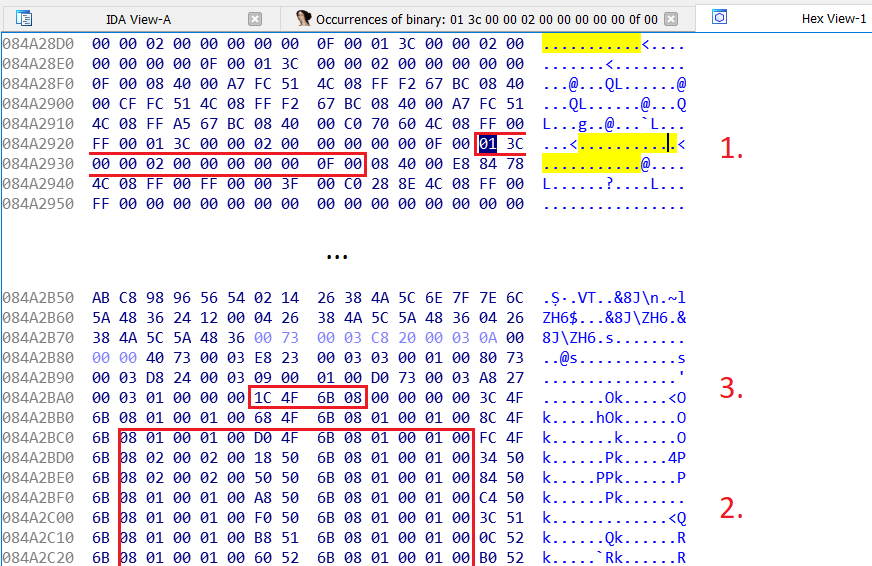
\includegraphics[width=0.5\textwidth]{Songtabelle}
	\end{center}
	\vspace{-10pt}
	\caption{Anfang der Songtabelle in Hex-Ansicht}
	\label{fig:hex-view}
	\vspace{-30pt}
\end{wrapfigure}

Um in IDA Pro die einzelnen Songs zu finden, wird zun\"achst nach der Songtabelle gesucht.

Diese findet man, indem man nach der HEX-Reihenfolge von ungenutzten Instrumenten sucht. Dabei handelt es sich um folgende Reihenfolge: 

\textbf{0x01, 0x3c, 0x00, 0x00, 0x02, 0x00, 0x00, 0x00, 0x00, 0x00, 0x0f, 0x00} (1.)

Wird die Sappy Sound Engine, wie bei Pok\'{e}mon Blattgr\"un, vom Spiel genutzt, sollten mehrere dieser Hex-Strings gefunden werden.
Scrollt man jetzt von der letzten \"ubereinstimmung der HEX-Reihenfolge aus weiter nach unten, sollten wir Spalten mit 0x00 und 0x08 auffinden. (2.)

Bei den ersten 4 Bytes welche mit 0x08 enden, handelt es sich um ein Zeiger auf den ersten Song im Spiel. (3.) Dieser befindet sich auf der ersten Position der Songtabelle. 
In der Abbildung \ref{fig:hex-view} handelt es sich dabei um den Zeiger auf die Adresse "`0x086B4F1C"'.

\vspace{15pt}

\begin{wrapfigure}{r}{0.5\textwidth}
	\vspace{-10pt}
	\begin{center}
		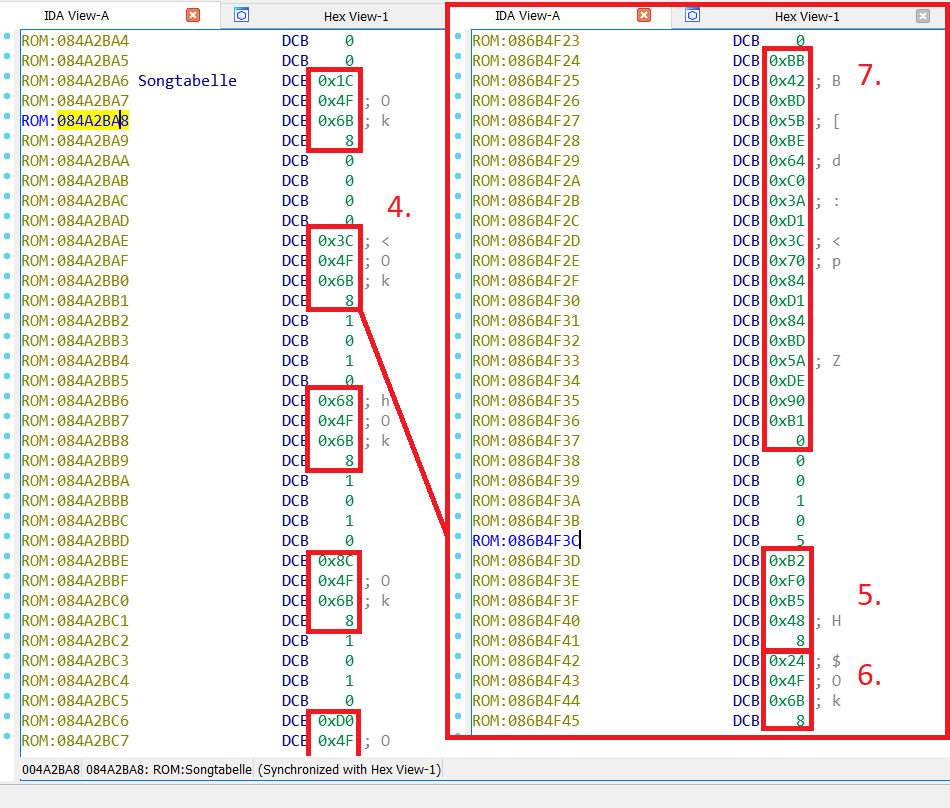
\includegraphics[width=0.5\textwidth]{SongtabellenHeader}
	\end{center}
	\vspace{-10pt}
	\caption{IDA-View der Songtabelle und erstem Song}
	\label{fig:IDA-view}
	\vspace{-40pt}
\end{wrapfigure}


Wird jetzt von der HEX-Ansicht auf die IDA-Ansicht gewechselt, k\"onnen die einzelnen Zeiger auf die Songs erkannt werden. (4.)
Folgt man nun einer dieser Zeiger landet man bei 0xB2, welches f\"ur eine Sprung-Anweisung steht, gefolgt von der Adresse des Instruments. (5.)

Nach der Adresse des Instruments folgt der Song-Header. (6.) Dieser f\"uhrt zum Trackformat, welcher immer mit der \enquote{Tempo}-Anweisung 0xBB Anf\"angt und mit der \enquote{Ende des Songs}-Anweisung 0xB1 endet. 

So wird in Abbildung \ref{fig:IDA-view} zun\"achst das Tempo (0xBB) auf 33 gesetzt und das 91. Instrument (0xBD) ausgew\"ahlt. Danach wird die Lautst\"arke (0xBE) auf 100 gesetzt und die Tonh\"ohe (0xC0) auf 58 variiert. Anschlie{\ss}end folgt eine Note mit automatischem Time-Out mit 60 112 132, dann ein Instrumenten Wechsel und endet mit der Ende des Songs Anweisung (0xB1). 

F\"ur genauere Bedeutung der Anweisungen, siehe \enquote{Sappy Track Format}-Tabelle \ref{table:TrackFormat}.

\newpage 

\begin{wrapfigure}{r}{0.5\textwidth}
	\vspace{-10pt}
	\begin{center}
		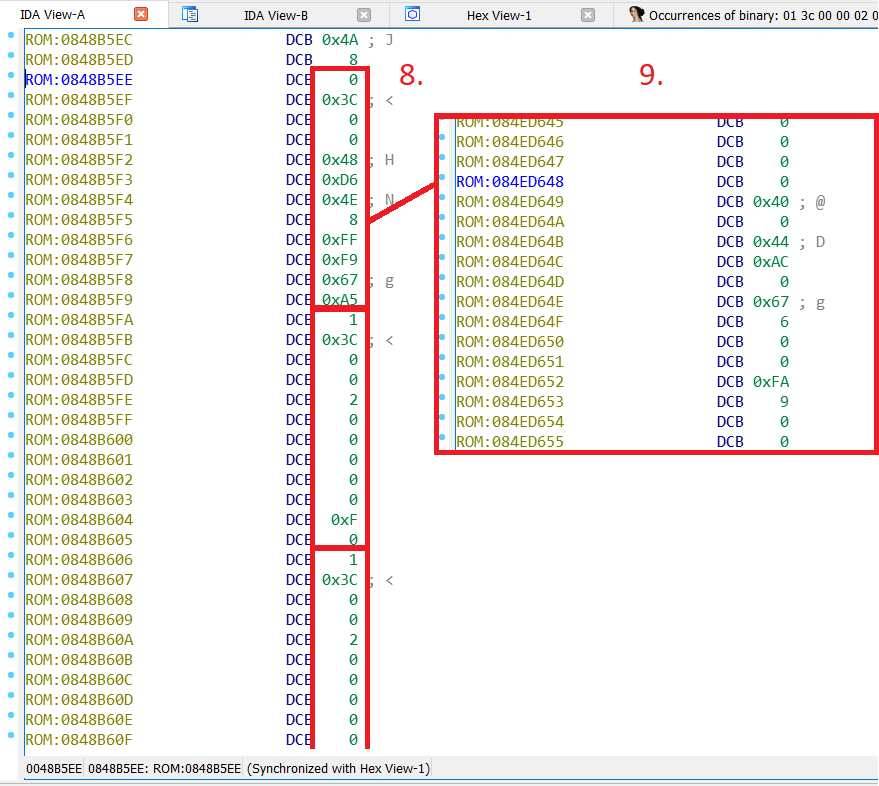
\includegraphics[width=0.5\textwidth]{Sampleformat}
	\end{center}
	\vspace{-10pt}
	\caption{IDA-View von Voice-Table und Sample-Format}
	\label{fig:Sampleformat}
	\vspace{-30pt}
\end{wrapfigure}

Folgt man der Adresse des Instrumentes, landet man bei der Voice-Tabelle. (8.) Dieser besteht typischerweise aus 127 Instrumenten, welche jeweils 12 Bytes pro Eintrag beanspruchen.

In der Abbildung \ref{fig:Sampleformat} erkennt man das es sich in diesem Beispiel um ein Sample handelt, dieser hat einen Zeiger auf die Sample Datei (0x084ED548). Weiterhin hat es einen Attack-Wert von 255 (0xFF), einen Decay-Wert von 249 (0xF9), einen Sustain-Level von 103 (0x67) und Release-Wert von 165 (0xA5) hat. Daraufhin Folgen zwei nicht genutzte Instrumente, welche man an der bereits Bekannten HEX-Reihenfolge erkennen kann.
F\"ur genauere Informationen, siehe "`Sappy Sample Instrument"'-Tabelle \ref{table:SampleInstrument}.

Die Sample Datei kommt mit einem 16-Byte Header (9.), gefolgt von einer variablen Datenl\"ange. So Handelt es sich in der Abbildung \ref{fig:Sampleformat} um ein geschleiftes Sample mit Pitch Adjustement
von 0xAC4400 (11025 Hz).

F\"ur genauere Informationen, siehe "`Sappy Sample Instrument"'-Tabelle \ref{table:SampleFormat}.

\vspace{15pt}
\begin{wrapfigure}{r}{0.5\textwidth}
	\vspace{-10pt}
	\centering
		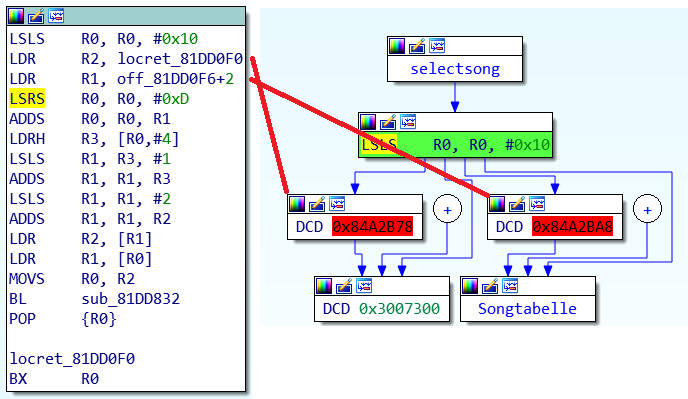
\includegraphics[width=0.75\linewidth]{SelectSong}
	\vspace{-10pt}
	\caption{IDA-Graph-View und Proximity-Browser-View f\"ur SelectSong Funktion}
	\label{fig:SelectSong}
\end{wrapfigure}

Die Song-Ausw\"ahl-Funktion f\"ur Sappy-Sound-Engine schaut in IDA aus wie in der Abbildung \ref{fig:SelectSong}. 

In der Proximity-Browser-View wird klarer, dass es sich um die Song-Ausw\"ahl-Funktion handelt, als in der Graph-View.

Diese kann man leicht finden, indem man nach Folgender HEX-Reihenfolge sucht:

\textbf{0x00, 0xB5, 0x00, 0x04, 0x07, 0x4A, 0x08, 0x49,
0x40, 0x0B, 0x40, 0x18, 0x83, 0x88, 0x59, 0x00,
0xC9, 0x18, 0x89, 0x00, 0x89, 0x18, 0x0A, 0x68,
0x01, 0x68, 0x10, 0x1C, 0x00, 0xF0}

\newpage
% ========== Chapter 2.3.3 ==========

\subsubsection{Sappy - \enquote{Audio-Reflektor}}
\AutorNgoc

\begin{figure}[h]
    \centering
    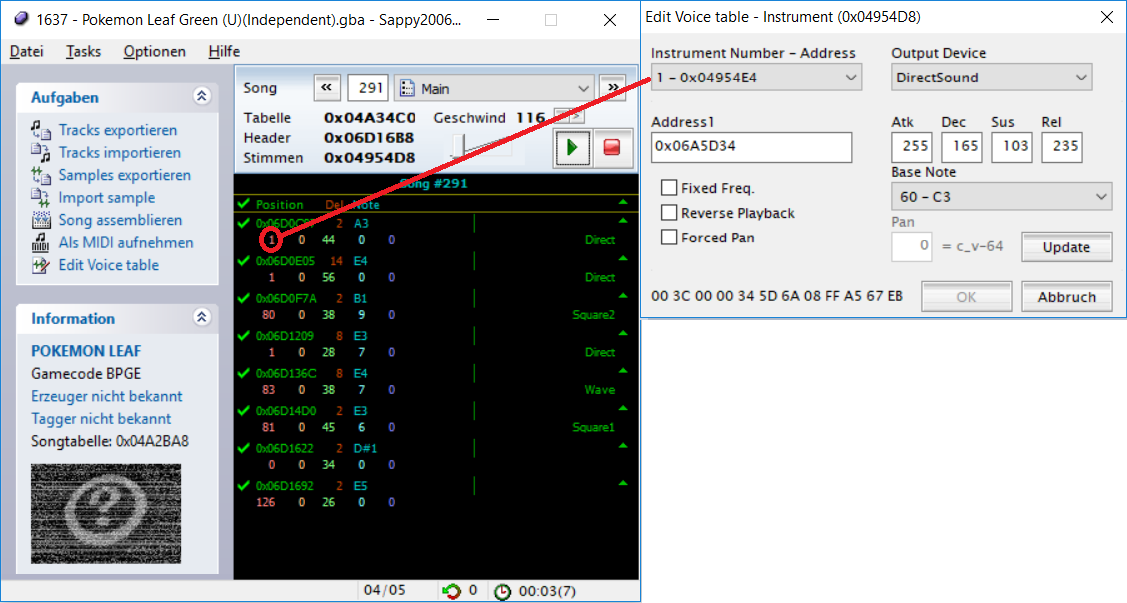
\includegraphics[width=\textwidth]{Sappy}
    \caption{Sappy Audio-Reflektor}
    \label{fig:Sappy}
\end{figure}

Sappy ist ein Programm um Musik von Game Boy Advance Spielen, falls sie die Sappy Sound Engine nutzen, zu extrahieren. Nach ausw\"ahlen eines Spieles werden die Songs und deren Instrumente automatisch gefunden.

Zu anderen Anwendungen geh\"oren das Abspielen von den gefundenen Songs, Bearbeitung, Entfernen und Hinzuf\"ugen von Tracks und Instrumente oder das Konvertieren in MIDI-Dateien.

So sieht man in der Abbildung \ref{fig:Sappy}, dass man im Vergleich zu IDA Pro viel einfacher die Gesuchten Daten findet. Diese werden unter anderem auch kompakter Angezeigt, welches man zum Beispiel an der Voice-Table merkt. So sieht man nicht nur alles auf einem Blick, sondern kann auch durch ein Drop-Down-Liste leicht zwischen Instrumente wechseln, oder die Werte \"andern.


\newpage

% ========== Chapter 3 ==========

\section{Emulation mittels mGBA} \label{EmulationMittelsMGBA}
\AutorDominikFlorian

% ========== Chapter 3.1 ==========

\subsection{Was ist der mGBA?}
\AutorDominik

\enquote{mGBA ist ein Open-Source Game Boy Advance Emulator, der von endrift entwickelt wurde. Von Grund auf neu geschrieben, zielt die Anwendung auf Geschwindigkeit, Genauigkeit und Portabilit\"at ab. Bis jetzt ist mGBA der umfassendste GBA-Emulator, der das \"altere Projekt VBA (Visual Boy Advance) und dessen Forks \"uberstanden hat [...]} \cite{mGBAWiki} Das K\"urzel \enquote{GBA} steht dabei f\"ur Game Boy Advance.

\enquote{mGBA ist eine neue Generation des Game Boy Advance Emulators. Das Projekt startete im April 2013 mit dem Ziel, schnell genug auf einer schw\"acheren Hardware zu laufen als andere Emulatoren, ohne auf Genauigkeit oder Portabilit\"at zu verzichten. Schon in der ersten Version liesen sich Spiele generell ohne Probleme spielen. mGBA ist seither immer besser geworden und r\"uhmt sich nun, der genaueste GBA-Emulator zu sein.

Weitere Ziele sind eine ausreichend genaue Emulation, um eine Entwicklungsumgebung f\"ur Homebrew-Software bereitzustellen, ein guter Workflow f\"ur Tool-Assist-Runner und ein moderner Funktionsumfang f\"ur Emulatoren, den \"altere Emulatoren m\"oglicherweise nicht unterst\"utzen.

mGBA ist unter der Mozilla Public License 2.0 lizenziert und [...] kann auf GitHub gefunden werden.} \cite{mGBAAbout}

\paratitle{F\"ur was steht das \enquote{m}?}
\enquote{[...] mGBA sollte urspr\"unglich miniGBA hei{\ss}en, aber als das Projekt wuchs, wurde der Begriff unpassend. Der Name sollte nur tempor\"ar sein, aber als die erste ver\"offentlichte Version n\"aher kam, konnte ich mir keine besseren Namen vorstellen. Andere Projektnamen f\"ur mGBA waren GBAc und Gerboa, aber nichts anderes blieb.} \cite{mGBAFaq}


% ========== Chapter 3.2 ==========

\subsection{Emulation des Game Boy Advance} \label{EmulationGameBoyAdvance}
\AutorDominikFlorian

Die Anwendung \enquote{mGBA} wurde von den Entwicklern mit dem GUI-Toolkit Qt realisiert. Qt erm\"oglicht die plattformunabh\"angige Entwicklung von Anwendungen mit grafischer Benutzeroberfl\"ache und basiert auf der Sprachen C und C++. Damit ist es Entwicklern auch m\"oglich, bereits realisierte Basis-Software problemlos zu integrieren.

% ========== Chapter 3.2.1 ==========

\subsubsection{Abgrenzung der Untersuchung}
\AutorFlorian

F\"ur die Untersuchung, wie der Emulator mit dem Betriebssystem interagiert, wird im Folgenden nur auf die daf\"ur ben\"otigten Klassen, Methoden und Konzepte eingegangen. Dabei liegt der Fokus ausschlie{\ss}lich auf Abl\"aufe die zur Emulation des Soundsystems notwendig sind.

\newpage
\subsubsection{Start des Emulators} \label{Emulator_Start}
\AutorDominik

Wie \"ublich beginnt auch beim mGBA die Anwendung in der globalen \verb|main|-Methode (\textit{\$/src/platform/qt/main.cpp}). Diese initialisiert den \textbf{ConfigController} mittels \verb|argc| und \verb|argv|. Anschlie{\ss}end wird eine neue Instanz der Klasse \textbf{GBAApp} ebenfalls mit \verb|argc| und \verb|argv|, sowie dem vorinitialisierten \verb|configController| initialisiert. Die weitere Logik der \verb|main|-Methode dient der Initialisierung und Lokalisierung einer \textbf{Window}-Instanz zur Anzeige der mGBA GUI. Die dabei erzeugte \textbf{Window}-Instanz wird w\"ahrenddessen dazu aufgefordert die Einstellungen aus dem bereits initialisierten \verb|configController| zu laden. Hierzu wird die Methode \verb|loadConfig()| der \textbf{Window}-Klasse verwendet.

Durch den Aufruf der \verb|loadConfig()|-Methode wird wiederum die Methode \verb|reloadConfig()| der \textbf{Window}-Klasse aufgerufen. Diese vermittelt unter anderen die aktuelle \textbf{mCoreConfig}-Struktur der \verb|m_config| (vom Typen \textbf{ConfigController}) an den \verb|m_controller| (vom Typen \textbf{GameController}) mittels \verb|setConfig()|-Methode der \textbf{GameController}-Klasse.

\paratitlecode{ConfigController}{/src/platform/qt/ConfigController.h \& .cpp}
Im Konstruktor der \textbf{ConfigController}-Klasse werden eventuell vorhandene Einstellungen aus einer \enquote{qt.ini} oder \enquote{config.ini} geladen und Standard-Werte der Membervariable \verb|m_opts| vom Typen der \textbf{mCoreOptions}-Struktur (\textit{\$/include/mgba/core/config.h}) festgelegt, siehe Snippet \ref{list:ConfigController_ctor}.

\vspace{5mm}
\begin{lstlisting}[language=C++, caption={Ausschnitt aus dem Konstruktor der ConfigController-Klasse}, label={list:ConfigController_ctor}]
    ...
	m_opts.audioSync = GameController::AUDIO_SYNC;
	m_opts.audioBuffers = 1536;
	m_opts.sampleRate = 44100;
	m_opts.volume = 0x100;
	...
\end{lstlisting}

Alle im \textbf{ConfigController} enthaltenen Einstellungen werden im Laufe der Anwendung je nach Bedarf entweder \"uber die \verb|options()|-Methode oder \"uber die \verb|config()|-Methode abgerufen. Dabei wird bei der ersten Methode eine \textbf{mCoreOptions}-Struktur (\textit{\$/include/mgba/core/config.h}) und bei der zweiten Methode eine \textbf{mCoreConfig}-Struktur (\textit{\$/include/mgba/core/config.h}) bereitgestellt. W\"ahrend die \textbf{mCoreConfig}-Struktur auschlie{\ss}lich eine Abstraktion der konfigurierten Werte, der Standardwerte und der \"uberschriebenen Werte bietet, stellt die \textbf{mCoreOptions}-Struktur alle verf\"ugbaren Einstellungen direkt als typisierte Felder bereit.

\paratitlecode{GBAApp}{/src/platform/qt/GBAApp.h \& .cpp}
Im Konstruktor der \textbf{GBAApp}-Klasse wird der lokale \verb|m_configController| mit dem \"ubergebenen initialisiert und der Treiber der \textbf{AudioProcessor}-Klasse mittels \verb|AudioProcessor.setDriver(...)| festgelegt. Der \textbf{AudioProcessor.Driver} (eine Enumeration) legt dabei fest, ob entweder die \textbf{AudioProcessor}-Spezialisierung \textbf{AudioProcessorQt} oder \textbf{AudioProcessorSDL} mittels \verb|AudioProcessor.create()|-Aufruf erstellt wird. Der zu verwendende \textbf{AudioProcessor.Driver} wird dabei durch den \textbf{ConfigController} \"uber die Option \enquote{audioDriver} bereitgestellt.

\newpage
\paratitlecode{Window}{/src/platform/qt/Window.h \& .cpp}
Im Konstruktor der \textbf{Window}-Klasse wird die lokale \verb|m_config| mit dem \"ubergebenen \textbf{ConfigController} (\verb|config|-Parameter) und der lokale \verb|m_inputController| initialisiert. Daraufhin wird eine neue Instanz der \textbf{GameController}-Klasse erzeugt, in der Membervariablen \verb|m_controller| gespeichert und der \verb|m_inputController| an die \textbf{GameController}-Instanz mittels \verb|m_controller.setInputController(...)| \"ubergeben. Weiter stellt der Konstruktor der \textbf{Window}-Klasse Verbindungen mittels Qt Signals \& Slots zwischen den folgenden Methoden her:

\begin{itemize}
    \item \verb|Window.audioBufferSamplesChanged| $\rightarrow$ \verb|m_controller::setAudioBufferSamples|
    \item \verb|Window.sampleRateChanged| $\rightarrow$ \verb|m_controller.setAudioSampleRate|
\end{itemize}

Als letzte Anweisung des Konstruktors wird die lokale \verb|setupMenu()|-Methode der \textbf{Window}-Klasse aufgerufen. Neben diversen Men\"ueintr\"agen erzeugt diese Methode auch Men\"upunkte zur Interaktion mit dem emulierten Soundsystem. Besonders interessant ist dabei auch der Men\"upunkt \enquote{Record output...}, welcher mittels Qt Signals \& Slots mit der Methode \verb|openVideoWindow()| der \textbf{Window}-Klasse verbunden wird. Bei Ausf\"uhrung der \verb|openVideoWindow()|-Methode wird eine neue Instanz der \textbf{VideoView}-Klasse erzeugt (falls nicht bereits geschehen) und die folgenden Methoden mittels Qt Signals \& Slots mit Methoden der \textbf{GameController}-Klasse verbunden. Zum Ende der Methode wird das \textit{QWidget} \textbf{VideoView} noch zur Anzeige gebracht.

\begin{itemize}
    \item \verb|VideoView.recordingStarted| $\rightarrow$ \verb|m_controller.setAVStream|
    \item \verb|VideoView.recordingStopped| $\rightarrow$ \verb|m_controller.clearAVStream|
\end{itemize}


\paratitlecode{VideoView}{/src/platform/qt/VideoView.h \& .cpp}
Bei der Instanziierung der \textbf{VideoView}-Klasse verwendet der Konstruktor die globale Methode \textbf{FFmpegEncoderInit} (\$/src/feature/ffmpeg/ffmpeg-encoder.c) zur Initialisierung der Membervariablen \verb|m_encoder|. Die f\"ur die Audio-/Videoausgabe verwendete Struktur vom Typen \textbf{FFmpegEncoder} (\$/src/feature/ffmpeg/ffmpeg-encoder.c) wird beim Aufruf der Instanzmethode \verb|startRecording()| der \textbf{VideoView}-Klasse mttels globaler \textbf{FFmpegEncoderOpen}-Methode so final konfiguriert, dass der Encoder die bei der Emulation anfallenden Audio-/Videodaten aufzeichnet. Zum Abschluss der \textbf{startRecording()}-Methode wird das Qt Signal \verb|recordingStarted| mit dem Feld \verb|d| vom Typen der Struktur \textbf{mAVStream} der \verb|m_encoder| Membervariablen als Parameter gesendet. Dieses Signal endet schlie{\ss}lich in einen Aufruf der \verb|setAVStream|-Methode der \textbf{GameController}-Instanz \verb|m_controller| der \textbf{Window}-Klasse.


\paratitlecode{GameController}{/src/platform/qt/GameController.h \& .cpp}
Im Konstruktor der \textbf{GameController}-Klasse wird die lokale \verb|m_audioProcessor| Membervariable mit dem Ergebnis des \verb|AudioProcessor.create()|-Aufrufs initialisiert. Daraufhin erfolgt das Setup der Membervariable \verb|m_threadContext| vom Typen der \textbf{mCoreThread}-Struktur. Hierbei wird unter anderen das \verb|startCallback|, \verb|cleanCallback| und das \verb|userData| Feld der Kontextvariablen entsprechend belegt. Abschlie{\ss}end werden die folgenden Methoden mittels Qt Signals \& Slots miteinander verbunden:

\begin{itemize}
    \item \verb|GameController.gamePaused| $\rightarrow$ \verb|m_audioProcessor.pause|
    \item \verb|GameController.gameStarted| $\rightarrow$ \verb|m_audioProcessor.setInput|
\end{itemize}

\newpage
\subsubsection{Initialisierung des \enquote{mCore}}
\AutorDominik

W\"ahlt der mGBA-Anwender im Men\"u den Punkt \enquote{Load ROM...}, wird hierf\"ur die Methode \verb|selectROM()| der \textbf{Window}-Klasse ausgef\"uhrt. Nach erfolgter Auswahl einer entsprechend unterst\"utzten Datei, wird die Methode \verb|loadGame(path)|  der lokalen \textbf{GameController}-Instanz (\verb|m_controller|) mit dem Pfad zur ausgew\"ahlten ROM-Datei aufgerufen. Diese f\"uhrt nach einigen Vorabaktionen die Methode \verb|openGame()| der \textbf{GameController}-Instanz aus. Mittels globaler \textbf{mCoreFind}-Methode (\textit{\$/src/core/core.c}) wird der vom Format der ROM-Datei abh\"angige \enquote{Core} ermittelt und erstellt.

\begin{figure}[h]
    \centering
    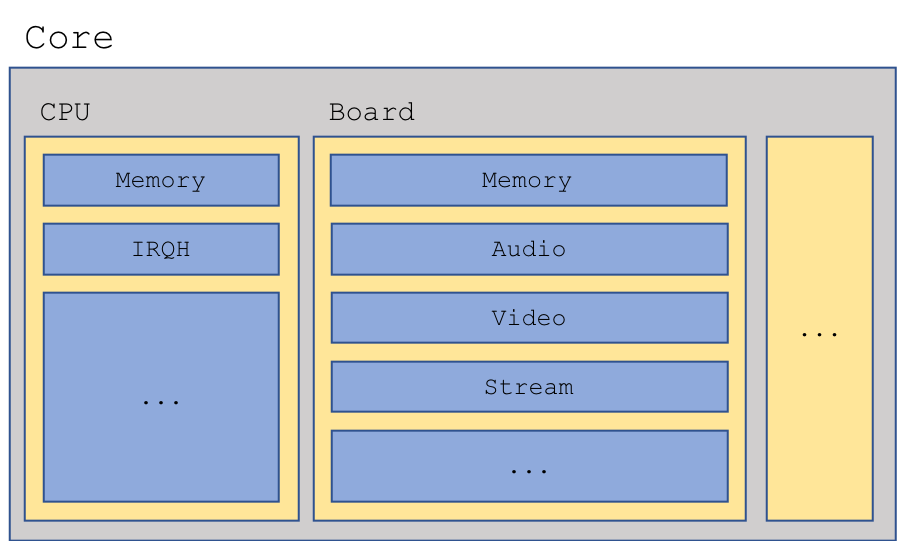
\includegraphics[width=0.7\textwidth]{Emulator_Core}
    \caption{Struktur des GBACore}
    \label{fig:mcore}
\end{figure}

Handelt es sich bei der ROM-Datei um ein Game Boy Advance (kurz \enquote{GBA}) Speicherabbild, wird die globale \textbf{GBACoreCreate}-Methode (\textit{\$/src/gba/core.c}) dazu verwendet den Speicher f\"ur die Struktur \textbf{GBACore} (\textit{\$/src/gba/core.c}) zu allokieren. Eine abstrakte Darstellung der Struktur ist in Abbildung \ref{fig:mcore} zu finden. Das dabei implizit allokierte \textbf{mCore}-Feld \verb|d| wird daraufhin mit diversen Funktionszeigern zu globalen Methoden mit dem Prefix \textbf{{\_}GBA} beziehungsweise \textbf{{\_}GBACore} initialisiert. Das auf diese Weise konfigurierte \verb|d|-Feld wird dann von der globalen \textbf{GBACoreCreate}-Methode zur\"uckgeliefert und im Feld \verb|mCoreThread.core| der lokalen Membervariable \verb|m_threadContext| der \textbf{GameController}-Instanz gespeichert.


\paratitlecode{{\_}GBACoreInit}{/src/gba/core.c}
Der erste der zuvor festgelegten Funktionszeiger der daraufhin verwendet wird ist der der Funktion auf die im Feld \verb|init| verwiesen wird. Nach Durchlaufen der globalen \textbf{GBACoreCreate}-Methode ist das die globale Methode \textbf{{\_}GBACoreInit}. Die globale Methode initialisiert die Felder \verb|cpu| und \verb|board| des \textbf{mCore}. Hierzu wird f\"ur das Feld \verb|cpu| die Struktur \textbf{ARMCore} (\textit{\$/include/mgba/internal/arm/arm.h}) und f\"ur das Feld \verb|board| die Struktur \textbf{GBA} (\textit{\$/include/mgba/internal/gba/gba.h}) verwendet. Nach der Initialisierung einzelner weiterer Felder wird dann die globale Methode \textbf{GBACreate} (\textit{\$/src/gba/gba.c}) mit den Verweis auf die zuvor initialisierte \verb|board|-Variable vom Typen der \textbf{GBA}-Struktur aufgerufen. Diese legt unter anderen als Wert f\"ur das \verb|init|-Feld des \verb|d|-Feldes vom Typen der \textbf{mCPUComponent}-Struktur der \verb|board|-Variablen die globale Methode \textbf{GBAInit} (\textit{\$/src/gba/gba.c}) fest. Anschlie{\ss}end wird in Folge der Aufrufe der globalen Methoden \textbf{ARMSetComponents} (\textit{\$/src/arm/arm.c}) und \textbf{ARMInit} (\textit{\$/src/arm/arm.c}) die zuvor auf dem \verb|init|-Feld des \verb|d|-Feldes der \verb|board|-Variablen die globale Methode \textbf{GBAInit} aufgerufen.

\newpage
\paratitlecode{GBAInit}{/src/gba/gba.c}
In dieser Low-Level Init-Routine werden alle virtuellen Hardwarekomponenten des \textbf{mCore} initialisiert und mit weiteren globalen Methoden verlinkt. Dazu geh\"ohrt unter anderen das Setup des Interrupt-Handlers, welcher \"uber das Feld \verb|irqh| des \verb|cpu|-Feldes der \textbf{GBA}-Instanz an die globale Methode \textbf{GBAInterruptHandlerInit} \"ubergeben wird. Nach der Initialisierung des Interrupt-Handlers folgt die Initialisierung des Speichers des \textbf{GBA} mittels globaler \textbf{GBAMemoryInit}-Methode. Darauf folgt das Setup der \enquote{Audio}-Peripherie des \textbf{GBA} mit Hilfe der globalen Methode \textbf{GBAAudioInit}.

\paratitlecode{GBAInterruptHandlerInit}{/src/gba/gba.c}
Die einzige Aufgabe dieser Methode ist es die \textbf{ARMInterruptHandler}-Struktur (\textit{\$/include/mgba/internal/arm/arm.h}) des \textbf{GBA} zu initialisieren. Hierzu legt die Methode entsprechende Funktionszeiger f\"ur die einzelnen Service-Routinen der Interrupt-Handler-Struktur fest.

\vspace{5mm}
\begin{lstlisting}[language=C++, caption={Ausschnitt aus der \textbf{GBAInterruptHandlerInit}-Methode}, label={list:GBAInterruptHandlerInit}]
    irqh->reset = GBAReset;
    irqh->processEvents = GBAProcessEvents;
    irqh->swi16 = GBASwi16;
    irqh->swi32 = GBASwi32;
    ...
\end{lstlisting}


\paratitlecode{GBAMemoryInit}{/src/gba/memory.c}
Neben den diversen Initialisierungsoperationen und Aufrufen weiterer Subroutinen zur Initialisierung des \verb|memory|-Feldes der \enquote{CPU} \"uber das \verb|cpu|-Feld des \textbf{GBA} legt auch diese Methode entsprechende Funktionszeiger f\"ur die einzelnen Speicherzugriffe auf der \textbf{ARMMemory}-Struktur (\textit{\$/include/mgba/internal/arm/arm.h}) fest. Die im folgenden Snippet gezeigten Zeilen sind f\"ur die Untersuchtung der Emulation des Soundsystems relevant.

\vspace{5mm}
\begin{lstlisting}[language=C++, caption={Ausschnitt aus der \textbf{GBAMemoryInit}-Methode}, label={list:GBAMemoryInit}]
    ...
    cpu->memory.load32 = GBALoad32;
    cpu->memory.load16 = GBALoad16;
    cpu->memory.load8 = GBALoad8;
    cpu->memory.loadMultiple = GBALoadMultiple;
    cpu->memory.store32 = GBAStore32;
    cpu->memory.store16 = GBAStore16;
    cpu->memory.store8 = GBAStore8;
    cpu->memory.storeMultiple = GBAStoreMultiple;
    cpu->memory.stall = GBAMemoryStall;
    ...
\end{lstlisting}

\newpage
\paratitlecode{GBAAudioInit}{/src/gba/audio.c}
In Abbildung \ref{fig:gbaaudio} ist die abstrakte Struktur der \textbf{GBAAudio} zu sehen. Das Feld \verb|psg| wird dabei f\"ur eine Instanz der \textbf{GBAudio} Struktur verwendet. Die Felder \verb|ch1| und \verb|ch2| dienen dabei als FIFOs f\"ur die je Kanal anliegenden Audiodaten. Die eigentlichen Kanalspezifischen Audioeinstellungen zur Tongenerierung finden sich jedoch im \verb|psg|-Feld. Dort wird je Kanaltyp die entsprechende Steuerung vorgenommen.

\begin{figure}[h]
    \centering
    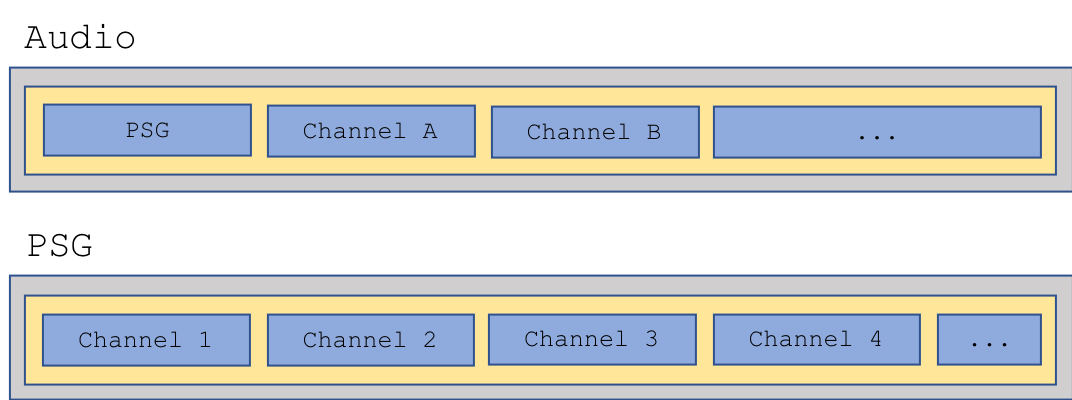
\includegraphics[width=0.7\textwidth]{Emulator_Audio}
    \caption{Struktur des GBAAudio}
    \label{fig:gbaaudio}
\end{figure}

Die globale \textbf{GBAAudioInit}-Methode ist f\"ur den vollen Setup der \textbf{GBAAudio}-Struktur (\textit{\$/include/mgba/internal/gba/audio.h}) der \textbf{GBA}-Instanz verantwortlich. Neben diversen Audio-Parametern werden auch ben\"otigte \textbf{mTimingEvent}-Strukturen initialisiert. Diese Event-Strukturen dienen dem Scheduler sp\"ater bei der quasi-parallelen Verarbeitung der Audiodaten. Die daf\"ur eigens definierten Events werden mit entsprechenden Callback-Routinen verlinkt, welche die verz\"ogerte / parallele Verarbeitung der Audiodaten durchf\"uhren. Zusammen mit der ebenfalls globalen Methode \textbf{GBAudioInit} werden w\"ahrend der Ausf\"uhrung der Methode die folgenden Events konfiguriert.

\begin{table}[h]
    \centering
    \begin{tabular}{ r | p{3cm} | c | p{7cm} }
        \textbf{Event} & \textbf{Priorit\"at} & \textbf{Kanal} & \textbf{Callback} \\
        \hline
        GB(A) Audio Sample & $0x18$ & & \verb|_sample| \\
        \hline
        GB  Audio Frame Sequencer & $0x10$ & & \verb|_updateFrame| \\
        \hline
        GB Audio Channel 1 & $0x11 \rightarrow 0x18$ & 1 & \verb|_updateChannel1|  \\
        \hline
        GB Audio Channel 2 & $0x12$ & 2 & \verb|_updateChannel2| \\
        \hline
        GB Audio Channel 3 & $0x13$ & 3 & \verb|_updateChannel3| \\
        \hline
        GB Audio Channel 3 Memory & $0x14$ & 3 & \verb|_fadeChannel3| \\
        \hline
        GB Audio Channel 4 & $0x15$ & 4 & \verb|_updateChannel4| \\
    \end{tabular}
    \caption{\"Ubersicht der Events der Soundkan\"ale des Game Boy Advance}
    \label{table:SoundEvents}
\end{table}

Die Verarbeitung der definierten Ereignisse zur Audioverarbeitung findet durch Aufruf der Methode im Feld \verb|processEvents| des \textbf{mCore} statt. Nach Durchlaufen der globalen \textbf{GBACoreCreate}-Methode ist das die globale Methode \textbf{{\_}GBAProcessEvents}. Die Ausf\"uhrung der Methode m\"undet in die \textbf{mTimingTick} welche letztendlich die \verb|callback|-Methoden (siehe Tabelle \ref{table:SoundEvents}) der einzelnen Ereignisse anst\"o{\ss}t.


\newpage
\subsubsection{Laden des ROM}
\AutorDominik

Wurde die Initialisierung des gesamten \textbf{mCore} abgeschlossen und die f\"ur die Emulation notwendigen Strukturen erzeugt, kann die eigentliche ROM Datei geladen werden. Ein Teil des Ladevorgangs ist dabei das Setup der zuvor geschaffenen \enquote{virtuellen} Peripherie. Dies geschieht anhand diverser \enquote{Setup}-Routinen. Wie dann letztlich der Inhalt der ROM geladen und interpretiert wird, h\"angt vom Format und dem Inhalt der ROM-Datei ab.

\paratitlecode{{\_}GBACoreSetAudioBufferSize}{/src/gba/core.c}
Anschlie{\ss}end wird mit Hilfe der globalen Methode \textbf{mCoreLoadForeignConfig} (\textit{\$/src/core/core.c}) die Konfiguration der \textbf{ConfigController}-Instanz, die durch die \textbf{Window}-Klasse an den \textbf{GameController} \"ubertragen wurde, auf den \textbf{mCore} des \verb|core|-Feldes der Membervariablen \verb|m_threadContext| angewendet. Hierbei wird unter anderen die Funktion auf die im Feld \verb|setAudioBufferSize| verwiesen wird aufgerufen. Nach Durchlaufen der globalen \textbf{GBACoreCreate}-Methode ist das die globale Methode \textbf{{\_}GBACoreSetAudioBufferSize}. Sie leitet den Aufruf direkt weiter an die globale Methode \textbf{GBAAudioResizeBuffer} unter Verwendung des \verb|audio|-Feldes der \textbf{GBAAudio}-Struktur des \verb|board|-Felds der \textbf{mCore}-Struktur.

\paratitlecode{{\_}GBACoreLoadConfig}{/src/gba/core.c}
Nachdem die Funktion auf die im Feld \verb|setAudioBufferSize| verwiesen wird aufgerufen wurde, wird von der globalen Methode \textbf{mCoreLoadForeignConfig} die allgemeine Funktion auf die im Feld \verb|loadConfig| verwiesen wird aufgerufen. Nach Durchlaufen der globalen \textbf{GBACoreCreate}-Methode ist das die globale Methode \textbf{{\_}GBACoreLoadConfig}. Sie \"ubernimmt im Wesentlichen die Konfiguration f\"ur das Mastervolume des \verb|audio|-Feldes der \textbf{GBAAudio}-Struktur des \verb|board|-Felds der \textbf{mCore}-Struktur.

\paratitlecode{{\_}GBACoreLoadROM}{/src/gba/core.c}
Auf die vorangegangene Konfiguration des \textbf{mCore} wird schlie{\ss}lich der ROM in den \enquote{Core} geladen. Hierzu verwendet die \textbf{GameController}-Instanz die Funktion auf die im Feld \verb|loadROM| verwiesen wird. Nach Durchlaufen der globalen \textbf{GBACoreCreate}-Methode ist das die globale Methode \textbf{{\_}GBACoreLoadROM}. Sie dient dem finalen Setup der virtuellen Hardwarekonfiguration des \textbf{mCore} sowie der Initialisierung des virtuellen Prozessspeichers im \verb|memory|-Feld des \verb|board|-Feldes der \textbf{mCore}-Instanz.

\paratitlecode{{\_}GBACoreSetAVStream}{/src/gba/core.c}
Bevor mit der eigentlichen Emulation begonnen wird, wird nun noch der Audio-/Videostream in Form der \textbf{mAVStream}-Struktur als \verb|m_stream|-Membervariable der \textbf{GameController}-Instanz an den \textbf{mCore} \"ubergeben. Diese geschieht durch Aufruf der Funktion auf die im Feld \verb|setAVStream| verwiesen wird. Nach Durchlaufen der globalen \textbf{GBACoreCreate}-Methode ist das die globale Methode \textbf{{\_}GBACoreSetAVStream}. Diese Methode geht hierbei lediglich dazu \"uber den \textbf{mAVStream}-Verweis im \verb|stream|-Feld des \verb|board|-Feldes der \textbf{mCore}-Instanz zu speichern.

\paratitlecode{{\_}GBACoreEnableAudioChannel}{/src/gba/core.c}
Aufgabe dieser globalen Methode ist es dem \verb|board|-Feld des \textbf{mCore} mittels gegebener Parameter zu konfigurieren. Das hierbei vorgenommene Setup bezieht sich auschlie{\ss}lich auf das \verb|audio|-Feld des \verb|board|-Felds vom Typen der \textbf{GBA}-Struktur. Die dabei vorgenommenen \"Anderungen beziehen sich somit nur auf Felder der \textbf{GBAAudio}-Struktur.


\newpage
\subsubsection{Starten des ROM}
\AutorDominik

\paratitlecode{mCoreThreadStart}{/src/core/thread.c}
Nach Abschluss des vollst\"andigen Setups des \textbf{mCore} wird die im \verb|m_threadContext.core| gespeicherte Instanz samt \verb|m_threadContext| an die globale Methode \textbf{mCoreThreadStart} \"ubergeben. Bevor aber die Methode den eigentlichen Thread erzeugt initialisiert sie diverse Mutex- sowie Condition-Instanzen zur Synchronisation der Thread-\"ubergreifenden Operationen. Von besonderer Bedeutung sind hierbei der Mutex \verb|audioBufferMutex| und die Condition \verb|audioRequiredCond|. Beide Felder sind Teil der \textbf{mCoreSync}-Struktur des \verb|theadContext|-Parameters vom Typen \textbf{mCoreThread}.

Sind alle Bedingungen f\"ur das Multithreading erf\"ullt, legt die Methode mittels globaler \textbf{ThreadCreate}-Methode (\textit{\$/include/mgba-util/platform/\{os\}/threading.h}) den Emulations-Thread an. Als \textbf{ThreadEntry} wird dabei die globale Methode \textbf{{\_}mCoreThreadRun} und als \verb|context|-Parameter ein Verweis auf den \textbf{mCoreThread} alias \verb|threadContext| verwendet. Der Verweis auf den so erzeugten Thread wird schlie{\ss}lich noch im \verb|thread|-Feld des \verb|threadContext|-Parameters gespeichert.

\paratitlecode{{\_}mCoreThreadRun}{/src/core/thread.c}
Zu Beginn der Methode werden noch weitere Methoden der \textbf{mCore}-Struktur ausgef\"uhrt. Eine dieser ist die Methode, die im Feld \verb|setSync| eingetragen ist. Nach Durchlaufen der globalen \textbf{GBACoreCreate}-Methode ist das die globale Methode \textbf{{\_}GBACoreSetSync}. Sie wird dazu verwendet um die \textbf{mCoreSync}-Struktur des \verb|m_threadContext->sync|-Feldes dem \textbf{mCore} bekannt zu machen. In ihr sind die bereits durch die \textbf{mCoreThreadStart}-Methode vorbereiteten Condition- und Mutex-Instanzen zur Thread-Synchronisation enthalten.

Bevor nun mit der eigentlichen Ausf\"uhrung des Prozesses begonnen wird, nimmt die globale \textbf{{\_}mCoreThreadRun} noch ein paar Vorkehrungen f\"ur die Threadinteraktion mittels Callback-Routinen vor. Darauf folgt der Aufruf der im Feld \verb|startCallback| des \verb|threadContext|-Parameters hinterlegten Methode. Dabei wird die durch die \textbf{GameContoller}-Klasse definierte anonyme Methode mit \verb|threadContext|-Parameter aufgerufen. W\"ahrend der Ausf\"uhrung des Start-Callbacks stellt der \textbf{GameController} sicher, dass im \textbf{mCore} (im \verb|core|-Feld des \verb|threadContext|-Parameters) die korrekten Audio-Kan\"ale ein- beziehungsweise ausgeschaltet sind. Hierzu verwendet der \textbf{GameController} die Funktion auf die im Feld \verb|enableAudioChannel| verwiesen wird. Nach Durchlaufen der globalen \textbf{GBACoreCreate}-Methode ist das die globale Methode \textbf{{\_}GBACoreEnableAudioChannel}.

\begin{wrapfigure}[18]{r}{0.40\textwidth}
    \centering
    \vspace{-7mm}
    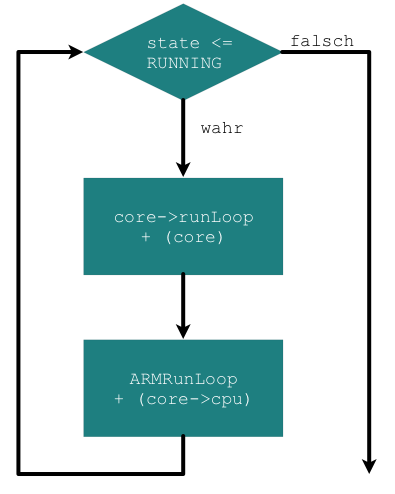
\includegraphics[width=0.35\textwidth]{Emulator_RunLoop}
    \caption{Ablauf der Methode}
    \label{fig:runloop}
\end{wrapfigure}

Abgeschlossen wird der Code der Callback-Routine mit dem dynamischen Ausl\"osen der Signale \textbf{gameStarted} und \textbf{startAudio} der \textbf{GameController}-Instanz die f\"ur den \"ubergebenen \verb|threadContext| zust\"andig ist. W\"ahrend \textbf{gameStarted} auf die \verb|setInput()|-Methode der \verb|m_audioProcessor|-Instanz im \textbf{GameController} weiterleitet, um den aktuellen \textbf{mCoreThread} der \textbf{AudioProcessor}-Instanz mitzuteilen, f\"uhrt der Aufruf des \textbf{startAudio}-Signals zum Aufruf der \verb|start()|-Methode der \verb|m_audioProcessor|-Instanz im \textbf{GameController}.

Wurden auch alle weiteren Callback-Routinen durchlaufen, beginnt die Ausf\"uhrung des Prozesses durch stetigen Aufruf der Funktion auf die im Feld \verb|runLoop| verwiesen wird. Nach Durchlaufen der globalen \textbf{GBACoreCreate}-Methode ist das die globale Methode \textbf{{\_}GBACoreRunLoop}. Dies geschieht solange, wie sich der Thread im Zustand kleiner/gleich \verb|THREAD_MAX_RUNNING| befindet. Der in Abbildung \ref{fig:runloop} gezeigte Programmablauf veranschaulicht den Ablauf.


\newpage
\subsubsection{Ausf\"uhrung des ROM}
\AutorDominik

Nach Durchlaufen der Setup-Phase bestehend aus dem Einrichten der notwendigen Strukturen und dem Laden des Prozessspeichers, kann der Inhalt des ROMs gem\"a{\ss} dem bekannten Instruction-Set eines ARM-Prozessors abgerarbeitet werden. Hierbei wird jede Anweisung im ROM sequentiell eine nach der anderen ausgewertet und ausgef\"uhrt. Die dabei im ROM beschriebenen Assembler Befehle f\"ur die ARM-Architektur, werden durch entsprechende Methoden abgearbeitet, welche das Verhalten der Plattform so emulieren, als ob der Prozess auf einem physikalichen ARM ausgef\"uhrt werden w\"urde.

\paratitlecode{{\_}GBACoreRunLoop}{/src/gba/core.c}
Die bereits im vorangegangenen Abschnitt erw\"ahnte globale Methode ist f\"ur die Ausf\"uhrung der einzelnen Assembler Anweisungen im geladenen ROM zust\"andig. Hierzu bedient sie sich der ebenfalls globalen Methode \textbf{ARMRunLoop} und \"ubergibt dieser dabei die Kontrolle \"uber die \enquote{CPU}.

\paratitlecode{ARMRunLoop}{/src/arm/arm.c}
Mit Hilfe der \"ubergebenen \enquote{CPU} in Form der \textbf{ARMCore}-Struktur f\"uhrt die Methode die Assembler-Anweisungen Schritt f\"ur Schritt aus. Dabei ber\"ucksichtigt sie die Anzahl der auszuf\"uhrenden Anweisungen in Abh\"angigkeit zur Ausf\"uhrung des n\"achsten Events. Bis es zur einer Abarbeitung von Events kommt wird je Zyklus die globale Methode \textbf{ARMStep} ausgef\"uhrt. Entspricht die Anzahl der vollzogenen Zyklen dem Zyklus eines anstehenden Events, wird die weitere Verarbeitung unterbrochen und dem Interrupt-Service-Routinen-Handler Zeit gegeben die anstehenden Events abzuarbeiten.

\paratitlecode{ARMStep}{/src/arm/arm.c}
Entsprechend der Natur von Software welche auf Hardware-Level in Form von Assembler-Befehlen ausgef\"uhrt wird, holt auch diese Methode stets den \textbf{OpCode} des als n\"achstes auszuf\"uhrenden Befehls aus dem Prefech-Speicher der \textbf{MMU}. Basierend auf den Wert des \textbf{OpCodes} wird aus einem global definierten und mittels Makros gef\"ulltem Array der Zeiger zur Funktion ermittelt, welche f\"ur die Emulation des Assembler-Befehls verantwortlich ist.

Die zur Ausf\"uhrung per Makro definierten Routinen vollziehen dabei nicht auschlie{\ss}lich einfache Delegationsarbeit zu global definierten Methoden deren Funktionszeiger in diversen Feldern des \textbf{mCore} gespeichert sind. Sie f\"uhren zus\"atzliche Pr\"ufungen, Vorabbedingungen und Nachbedingungen sowie weitere Operationen aus die f\"ur die korrekte Interaktion mit dem Prozess und dem emulierten Speicher notwendig sind. Die Operationen stellen dabei ein Mindestma{\ss} an Korrektheit der ausgef\"uhrten Assembler-Befehle vor und nach Ausf\"uhrung der Callback-Routinen sicher - falls f\"ur den Befehl eine solche vorliegt.

\vspace{5mm}
\begin{lstlisting}[language=C++, caption={Ausschnitt aus der \textbf{ARMStep}-Methode}, label={list:ARMStep}]
    uint32_t opcode = cpu->prefetch[0];
	cpu->prefetch[0] = cpu->prefetch[1];

	cpu->gprs[ARM_PC] += WORD_SIZE_ARM;
	
	LOAD_32(
	    cpu->prefetch[1],
	    cpu->gprs[ARM_PC] & cpu->memory.activeMask,
	    cpu->memory.activeRegion);
    ...
	uint32_t instructionIndex = ((opcode >> 16) & 0xFF0) | ((opcode >> 4) & 0x00F);
	
	ARMInstruction instruction = _armTable[instructionIndex];
	instruction(cpu, opcode);
\end{lstlisting}

Die Signatur einer \textbf{ARMInstruction} ist dabei so einfach wie m\"oglich gehalten. So erwartet jede Funktion des Instruction-Sets einen Verweis auf die \enquote{CPU}, auf der die Anweisung ausgef\"uhrt werden soll, sowie den zur \textbf{ARMInstruction} gef\"uhrten \textbf{OpCode}.

Ein Beispiel f\"ur so eine Makrodefinition kann im folgenden betrachtet werden. Die eigentliche Verarbeitung mittels globaler Callback-Routine findet in Zeile 5 des Snippets \ref{list:ARMInstruction_STRT} statt.

\vspace{5mm}
\begin{lstlisting}[language=C++, caption={ARM Instruction Makro f\"ur \textbf{STRT}}, label={list:ARMInstruction_STRT}]
    DEFINE_LOAD_STORE_T_INSTRUCTION_ARM(STRT,
	    enum PrivilegeMode priv = cpu->privilegeMode;
	    int32_t r = cpu->gprs[rd];
	    ARMSetPrivilegeMode(cpu, MODE_USER);
	    cpu->memory.store32(cpu, address, r, &currentCycles);
	    ARMSetPrivilegeMode(cpu, priv);
	    ARM_STORE_POST_BODY;)
\end{lstlisting}

Gem\"a{\ss} vorangegangenem Snippet \ref{list:GBAMemoryInit} sah man in Zeile 6 der Methode \textbf{GBAMemoryInit}, dass das Feld \verb|store32| mit der globalen Methode \textbf{GBAStore32} belegt wurde, welche an dieser Stelle bei der Ausf\"uhrung des Assembler-Befehls \textbf{STRT} (unter anderen) ausgef\"uhrt wird.

Der Aufruf der gloablen \textbf{GBAStore32} (\textit{\$/src/gba/memory.c}) Methode f\"uhrt dann zum Beispiel zum Aufruf der ebenfalls globalen Methode \textbf{GBAIOWrite32} (\textit{\$/src/gba/memory.c}) welche wiederum zum Beispiel in eine der f\"ur das Soundsystem folgenden relevanten Methoden m\"unden kann:

\begin{itemize}
    \item \textbf{GBAAudioWriteWaveRAM} (\textit{\$/src/gba/audio.c})
    \item \textbf{GBAAudioWriteFIFO} (\textit{\$/src/gba/audio.c})
\end{itemize}


% ========== Chapter 3.3 ==========

\subsection{Emulation des Soundsystems} \label{EmulationSoundsystem}
\AutorDominik

Damit die vom ROM liegenden beziehungsweise vom Prozess generierten Audiodaten auch mittels \textbf{mAVStream} in der \textbf{VideoView} sowie durch das \textbf{AudioDevice} verarbeitet werden bedient sich mGBA verschiedener Methoden. Zur Ausgabe \"uber den \textbf{mAVStream} greift der Callback des \enquote{GB(A) Audio Sample}-Events (die globale \textbf{{\_}sample} Methode) direkt auf das \verb|stream|-Feld \"uber den \textbf{GBA}-Verweis des Feldes \verb|p| in der \textbf{GBAAudio}-Struktur zu. Hierbei bedient sich die \textbf{{\_}sample} Methode des dort eingetragenen Callbacks im Feld \verb|postAudioBuffer| und ruft somit eine Methode der vom mGBA verwendeten \textbf{FFmpeg}-Library auf um die Audiodaten im Stream abzulegen.


% ========== Chapter 3.3.1 ==========

\subsubsection{Audioverarbeitung im Assembler}
\AutorDominik

Im Rahmen der Untersuchungen wurde festgestellt, dass die Audiodaten entweder vorab im ROM vorliegen oder im Assembler generiert werden. Ausschlaggebend f\"ur die Audioverarbeitung ist dabei die korrekte Interaktion mit den zust\"andigen Registern. Im Allgemeinen wird immer zuerst ein Sample mit zugeh\"origen Audiosetup in die daf\"ur vorgesehenen Register geschrieben. Nachdem alle f\"ur ein Sample notwendigen Konfigurationen getroffen wurden, wird \"uber das Master Control Register die Audioausgabe angesto{\ss}en.

Wurde ein Sample vom \enquote{AudioProcessor} verarbeitet, kann das Programm den n\"achsten Sample in die Register laden und wiederholt die Verarbeitung ansto{\ss}en. Im Wesentlichen basiert die Audioverarbeitung im Assembler prim\"ar darauf, dass Samples entweder getaktet oder mittels FIFO bereitgestellt werden. Liegen die Daten bereit, werden diese anschlie{\ss}end als \enquote{bereit zur Ausgabe} markiert. Erst nach erfolgter Ausgabe wird der n\"achste Sample bereitgestellt, beziehungsweise noch w\"ahrend der Ausgabe aus einem FIFO dieser kontinuierlich weiter bef\"ullt.

Die f\"ur die Verarbeitung notwendigen Register wurden bereits im Abschnitt \ref{Hardwareumgebung} genannt. Essentiell sind aufgrund der eben beschriebenen Operationen Assembler-Befehle, die zum Laden und Speichern von Daten in und aus den besagten Registern notwendig sind. Ein Beispiel-Befehl ist hierf\"ur der \textbf{STRT}-Befehl, dessen Interpretation im Bezug auf die \textbf{ARMStep}-Methode erkl\"art wurde. Betrachtet man dessen Umsetzung vom Assembler-Code zum C-Code, dann erkennt man die logischen Abl\"aufe, welchen Einfluss ein Assembler-Befehl auf die Ausf\"uhrung des ROMs im Emulator hat.


% ========== Chapter 3.3.2 ==========

\subsubsection{Weiterverarbeitung im Emulator}
\AutorDominik

Im Kontext der von der \textbf{VideoView} unabh\"angigen Abl\"aufe der Audiodatenverarbeitung stellt man fest, dass die Verarbeitung direkt \"uber den Speicher des \textbf{mCore} stattfindet. Da aber der Speicher vom Emulations-Thread verwendet wird, kann der Main-Thread nicht ohne weiteres auf diesen zugreifen. An dieser Stelle kommen die in der \textbf{mCoreThreadStart} initialisierte Condition \verb|audioRequiredCond| sowie der Mutex \verb|audioBufferMutex| ins Spiel. W\"ahrend der Callback des \enquote{GB(A) Audio Sample}-Events (die globale \textbf{{\_}sample} Methode) die globale Methode \textbf{mCoreSyncProduceAudio} verwendet, nutzt im Main-Thread die \textbf{AudioDevice}-Instanz des verwendeten \textbf{AudioProcessor}'s die globale Methode \textbf{mCoreSyncConsumeAudio}.

Letztere verwendet die \textbf{mCoreSyncConsumeAudio} Methode \underline{nach} dem Zugriff auf die Audiodaten im Speicher, w\"ahrend \underline{vor} dem Zugriff weitere Zugriffe durch den Prozess mittels Aufruf der globalen \textbf{mCoreSyncLockAudio} Methode blockiert werden. Erst der Aufruf der \textbf{mCoreSyncConsumeAudio} Methode gibt den Zugriff auf den Audiodaten-Speicher wieder frei. Der grobe Ablauf des Synchronisation im \textbf{AudioDevice} kann in Snippet \ref{list:AudioDevice_LockConsume} betrachtet werden.

\vspace{5mm}
\begin{lstlisting}[language=C++, caption={AudioDevice - \enquote{Lock / Consume}}, label={list:AudioDevice_LockConsume}]
	mCoreSyncLockAudio(&m_context->sync);
	...
	blip_read_samples(
            m_context->core->getAudioChannel(m_context->core, 0),
            &reinterpret_cast<GBAStereoSample*>(data)->left,
            ...);
    ...
    mCoreSyncConsumeAudio(&m_context->sync);
\end{lstlisting}

Ebenso wie das \textbf{AudioDevice} den Zugriff auf die Audiodaten blockiert, w\"ahrend diese gelesen werden, so blockiert auch die \textbf{{\_}sample}-Methode den Zugriff auf diese mit einem ebenfalls vorgeschalteten Aufruf der \textbf{mCoreSyncLockAudio} Methode. Nach der Bearbeitung der Audiodaten werden diese schlie{\ss}lich mit Aufruf der globalen \textbf{mCoreSyncConsumeAudio} Methode f\"ur den Zugriff wieder freigegeben. Wie in etwa die Methode bei der Synchronisation vorgeht, kann im folgenden Snippet \ref{list:Sample_LockConsume} nachvollzogen werden.

\vspace{5mm}
\begin{lstlisting}[language=C++, caption={{\_}sample - \enquote{Lock / Consume}}, label={list:Sample_LockConsume}]
	mCoreSyncLockAudio(audio->p->sync);
    ...
    blip_add_delta(audio->left, audio->clock, sampleLeft - audio->lastLeft);
    ...	
	bool wait = produced >= audio->samples;
	mCoreSyncProduceAudio(audio->p->sync, wait);
	...
\end{lstlisting}


% ========== Chapter 3.3.3 ==========

\newpage

\subsection{Interaktion mit dem Betriebssystem}

\subsubsection{Start des Emulators}
\AutorFlorian

Im Kapitel \ref{Emulator_Start} wurde bereits der Ablauf bis zur Erstellung der AudioProcessor-Klasse, sowie das Setzten des Treibers beschrieben. Auf diesen Ablauf wird im Folgenden nun aufgesetzt. In dieser Arbeit
wird der \enquote{Qt Multimedia} Treiber untersucht und schlie{\ss}t somit die Betrachtung des SDL-Treibers aus.

Startet der Benutzer den mGBA, wird unter Verwendung des zuvor gesetzten Treibers, eine neue Instanz von AudioProcessor erstellt. In diesem Fall wird die AudioProcessor::create() Methode aufgerufen und w\"ahlt \"uber ein Switch Statement den Konstruktor von AudioProcessorQt aus und liefert eine neue Instanz zur\"uck. Dieser verf\"ugt \"uber keine Logik und ist demnach leer. F\"ur die weitere Untersuchung folgt ein Klassendiagramm der wesentlichen Klassen auf Seitens der Qt-Anwendung.

\begin{figure}[h!]
    \centering
    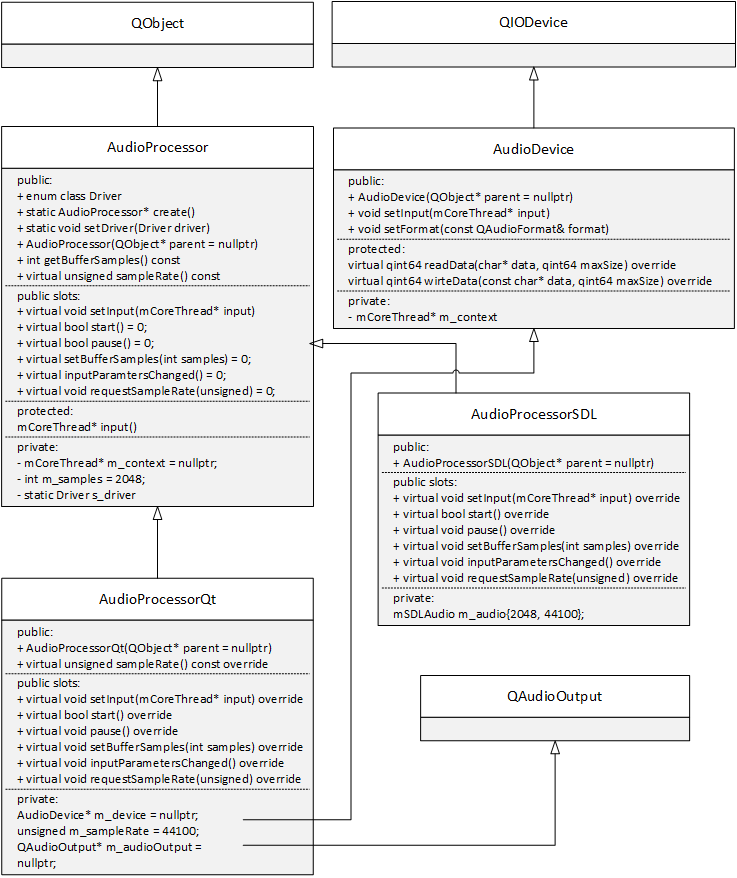
\includegraphics[width=0.7\textwidth]{QT_Klassendiagramm}
    \caption{Audioklassen in der QT-Anwendung}
    \label{fig:qtclassdiagramm}
\end{figure}

\newpage

\paratitlecode{AudioProcessor-Klasse}{/src/platform/qt/AudioProcessor.cpp}
Die Klasse AudioProcessor erbt von QObject, ist eine abstrakte Klasse und definiert ein Interface f\"ur die Klassen AudioProcessorQt und AudioProcessorSDL. QObject ist die Basisklasse aller Qt Objekte und im Bezug auf
die Objektmodellierung somit das Herzst\"uck von Qt. 

\textbf{AudiProcessor::getBufferSamples} liefert die Anzahl der, intern in der Variablen m\_samples gespeicherten, Samples zur\"uck. Diese wird initial auf den Wert 2048 gesetzt. m\_samples kann mit dem Aufruf von \textbf{AudiProcessor::setBufferSamples} ge\"andert werden. Es folgen abstrakte Methoden und Slots. Diese werden in der Klasse \textbf{AudioProcessorQt} \"uberschrieben.

Weiterhin beinhaltet die Klasse eine Variable m\_context. Diese stellt einen Zeiger auf den mCoreThread dar und kann mit der Methode \textbf{AudioProcessor::setInput(mCoreThread* input)} gesetzt werden. 

Unter Verwendung einer selbst kompilierten Version von mGBA, mit Log-Ausgaben, konnte nach dem Erstellen der AudioProcessorQt-Klasse festgestellt werden, dass 
die \textbf{AudioProcessorQt::inputParameterChanged} Methode f\"unfmal aufgerufen wird. Gefolgt von einem Aufruf der \textbf{AudioProcessorQt::requestSampleRate} und dreimal der \textbf{AudioProcessorQt::inputParameterChanged} Methode. Ein weiterer Aufruf der \textbf{AudioProcessorQt::requestSampleRate} Methode folgt. Interessant an dieser Stelle ist, dass jeder Aufruf der zuvor aufgef\"uhrten Methoden bereits bei der \"Uberpr\"ufung ob ein \textbf{AudioDevice} vorhanden ist, scheitert. 
Daraus folgt, dass an dieser Stelle keine \"Anderungen vorgenommen werden. %Eine genauere Betrachtung der aufger\"uhrten Methoden folgt im folgenden Kapitel.

\subsubsection{Einstellungen \"uber die mGBA GUI} \label{kapitelEinstellungenMGBA}
\AutorFlorian

Der mGBA ist gestartet und die\textbf{AudioProcessorQt} wurde erstellt. Der Benutzer kann nun \"uber die Men\"uleiste Werkzeuge$\rightarrow$Einstellungen$\rightarrow$Audio/Video auf die Audio und Video Einstellungen zugreifen.

\begin{figure}[h!]
    \centering
    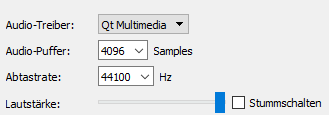
\includegraphics[width=0.7\textwidth]{Audioeinstellungen}
    \caption{Audioeinstellungen im mGBA}
    \label{fig:audioeinstellungen}
\end{figure}

In Abbildung \ref{fig:audioeinstellungen} sind die f\"ur dem Benutzer m\"oglichen Einstellungen im Bezug auf das Audiosystem dargestellt. Der Audio-Treiber kann entweder auf Qt Multimedia oder SDL eingestellt werden.
Der Audio-Puffer bietet die g\"angisten Anzahl an Samples von 512 bis 4096. Kann aber auch benutzerspezifische eingestellt werden. Weiterhin kann die Abtastrate gesetzt werden. Auch hier sind die g\"angigsten Raten vorgeschlagen, k\"onnen
aber auch frei gesetzt werden. Schlie{ss}lich folgt die Lautst\"arkeneinstellung.

Wie schon zu erahnen ist, wird nach einer Ver\"anderung des Audio-Treibers der Destruktor der zuvor gew\"ahlten Klasse aufgerufen und ein erneuter Aufruf der \textbf{AudioProcessor::create} Methode erzeugt eine neue AudioProcessor Instanz.
Anlie{\ss}end wird die Methode \textbf{AudioProcessor::setBufferSamples} aufgerufen. Als \"Ubergabeparameter erh\"ahlt diese den Wert aus dem Feld Audio-Puffer und setzt diesen in die interne Variable m\_samples.
\newpage


\subsubsection{Starten des ROM}
\AutorFlorian

W\"ahlt der Benutzer eine neue ROM aus und startet diese, wird zun\"achst die \textbf{AudioProcessor::setInput} Methode aufgerufen. Diese setzt den Zeiger auf den m\_coreThread zur internen Variablen m\_context. Es folgt der Aufruf der
\textbf{AudioProcessorQt::start} Methode.

\paratitlecode{AudioProcessorQt::start()}{/src/platform/qt/AudioProcessorQt.cpp}
Im ersten Schritt wird \"uberpr\"uft, ob der m\_coreThread bereits gesetzt wurde. Im n\"achsten Schritt wird der internen Variablen \textbf{m\_device} ein neue Instanz von \textbf{AudioDevice} zugewiesen.

Die Klasse \textbf{AudioDevice} stellt das Bindeglied zwischen AudioProcessorQt und dem mCoreThread dar. \textbf{AudioDevice} erbt von QIODevice. QIODevice ist ein Interface f\"ur alle I/O Ger\"ate und kann deshalb nicht direkt instanziiert werden.
Wird von dieser Basisklasse abgeleitet, m\"ussen die Methoden \textbf{readData} und \textbf{writeData} \"uberschrieben werden. Zus\"atzlich muss die Methode \textbf{setOpenMode} mit dem gew\"unschten Modus im Konstruktor aufgerufen werden. In diesem Fall wird der Parameter \enquote{ReadOnly} \"ubergeben. Daraus resultiert ein nur lesbares QIODevice. Weiterhin wird auch hier der mCoreThread \"ubergeben und gesetzt. Die bereits erw\"ahnte Methode \textbf{writeData} spielt hier keine Rolle, da nicht auf das Ger\"at geschrieben werden darf. Sie muss jedoch \"uberschrieben werden aber beinhaltet nur eine Warnung. Eine genauere Betrachtung der Funktionsweise der Klasse folgt.

Es folgt das Erzeugen einer neuen Instanz von QAudioFormat. Die Klasse \textbf{QAudioFormat} speichert Informationen \"uber Audio-Stream Parameter.

\vspace{5mm}
\begin{lstlisting}[language=C++, caption={Ausschnitt aus AudioProcessorQt::start()}, label={list:FormatAudioProcessorQt}]
    QAudioFormat format;
    format.setSampleRate(m_sampleRate); // m_sampleRate = 44100
    format.setChannelCount(2);			// 2 bedeutet Stereo 1 Mono
    format.setSampleSize(16);			// Typischerweise 8 oder 16
    format.setCodec("audio/pcm");		// Linear PCM
    format.setByteOrder(QAudioFormat::Endian(QSysInfo::ByteOrder));

    // Little- oder Big-Endian
    format.setSampleType(QAudioFormat::SignedInt);

    // Sample Typ
    m_audioOutput = new QAudioOutput(format, this);
    m_audioOutput->setCategory("game");
\end{lstlisting}
  
Wie bereits am Ende von Snippet \ref{list:FormatAudioProcessorQt} zu sehen, wird eine neue Instanz der Klasse \textbf{QAudioOutput} erzeugt und in die interne Variable \textbf{m\_audioOutput} geschrieben. 
Dem Konstruktor der Klasse \textbf{QAudioOutput} wird das zuvor erstellte Format \"ubergeben.

\textbf{QAudioOutput} stellt ein Interface zur Verf\"ugung mit dem Audiodaten zu einem Audio-Ger\"at
gesendet werden k\"onnen(z.B. Lautsprecher, Kopfh\"orher usw.) Die \textbf{setCatecory} Methode setzt den Modus auf \enquote{game}. Einige Plattfomren k\"onnen Audio-Streams in Kategorien gruppieren.
N\"utzlich ist dieser Methodenaufruf, da unter Windows der mGBA nun im Lautst\"arken Mixer angezeigt wird.

Durch den Methodenaufruf \textbf{m\_device$\rightarrow$setInput} wird der Klasse \textbf{AudioDevice} der \textbf{mCoreThread} \"ubergeben. Daraufhin wird die \textbf{m\_device$\rightarrow$setFormat} Methode, mit einer Referenz auf
das Format von \textbf{m\_audioOutput} als \"Ubergabeparameter, aufgerufen.

\newpage
\paratitlecode{AudioDevice::setFormat(const QAudioFormat\& format)}{/src/platform/qt/AudioDevice.cpp} 
Wie gewohnt wird zun\"achst \"uberpr\"uft, ob der \textbf{mCoreThread} vorhanden ist. Im n\"achsten Schritt wird ein Multiplikator errechnet. Dieser wird abh\"angig von der eingestellten FPS berechnet. Bei 60 FPS betr\"agt dieser
0,995458. Anschli{\ss}end werden die im \textbf{mCoreThread} befindlichen Audio-Speicherbereiche gesperrt. Nun werden die Frequenzen der beiden Audiokan\"ale im \textbf{mCoreThread} mit den Frequenzen, multipliziert mit dem zuvor errechneten
Multiplikator, des \textbf{m\_audioOutput} synchronisiert. Mit dem entsperren der Speicherbereiche endet die Methode.

Zur\"uck in der \textbf{AudioProcessorQt::start} Methode wird mit dem Aufruf von \textbf{m\_audioOutput$\rightarrow$start(m\_device)} die Audioausgabe gestartet. Schlie{\ss}lich wird der Status des \textbf{m\_audioOutput} auf aktive gesetzt.
Konnte der Status erfolgreich auf aktiv gesetzt werden, liefert \textbf{AudioProcessorQt::start} \enquote{true} zur\"uck.
 
\subsubsection{Transferirrung der Audiodaten}
\AutorFlorian

Wie bereits im vorangegangenen Kapitel erw\"ahnt, wird der \textbf{m\_audioOutput$\rightarrow$start} Methode das \textbf{AudioDevice} \"ubergeben. Dies bewirkt, dass die Klasse \textbf{QAudioOutput} jetzt von der Klasse \textbf{AudioDevice} 
Daten f\"ur die Audioausgabe liest und diese an die Systemausgabe weiterleitet. Einmal gestartet, l\"auft die Audioausgabe kontinuierlich weiter. Nur ein Aufruf der Methode \textbf{AudioProcessorQt::pause} stoppt die Ausgabe.

Die Klasse \textbf{QAudioOutput} ruft nun selbstst\"andig  in gewissen Zeitabst\"anden die \textbf{AudioDevice::readData} Methode auf und \"ubergibt einen Zeiger in dem die Daten zur Ausgabe eingelesen werden sollen und dessen Gr\"o{\ss}e.


\paratitlecode{AudioDevice::readData(char* data, qint64 maxSize)}{/src/platform/qt/AudioDevice.cpp}
Wie bereits erw\"ahnt, muss diese Methode \"uberschrieben werden. Zu Beginn wird \"uberpr\"uft ob die maximal zul\"assige Gr\"o{\ss}e des \"ubergebenen Puffers nicht \"uberschritten ist und der \textbf{m\_coreThread} vorhanden ist.
Nun wird, wie auch in der \textbf{AudioDevice::setFormat} Methode, der Speicherbereich im \textbf{m\_coreThread} in dem die Audiodaten gespeichert sind gesperrt.
Mit dem Methodenaufruf \textbf{blip\_samples\_avail} wird die Anzahl der verf\"ugbahren Samples im \textbf{m\_coreThread} abgefragt. \"Uberschreitet die Anzahl der Samples die Gr\"o{\ss}e des Puffers, geteilt durch die 
Strukturgr\"o{\ss}e \textbf{GBAStereoSample}, wird die Anzahl der verf\"ugbahren Samples auf die Puffergr\"o{\ss}e, geteilt durch die Strukturgr\"o{\ss}e \textbf{GBAStereoSample}, reduziert.

Jetzt k\"onnen die Samples aus dem \textbf{m\_coreThread} gelesen werden. Dies geschieht durch den Methodenaufruf von \textbf{blip\_read\_samples} f\"ur den linken und den rechten Kanal. 
Dazu wird der \"ubergebene Puffer auf die Struktur \textbf{GBAStereoSample} gecastet und \"ubergeben. Ein Entsperren des zuvor gesperrten Speicherbereichs und das Zur\"uckgeben der Anzahl gelesener Daten beendet die Methode
\textbf{AudioDevice::readData}. Die im Puffer befindlichen Daten werden nun in der Klasse \textbf{QAudioOutput} verarbeitet und zum Systemausgang weitergeleitet.


% ========== Chapter 4 ==========

\newpage
\section{Zusammenfassung} \label{Zusammenfassung}

% ========== Chapter 4.1 ==========

\subsection{Inhalt des Dokumentes}
\AutorDominik

Entsprechend der Aufgabenstellung zur Studienarbeit f\"ur die Vorlesung Computer Architektur haben die drei Studenten Ngoc Luu Tran, Florian Boemmel und Dominik Scharnagl in kooperativer Arbeit die Aufgabenstellung bearbeitet. Im Rahmen dieser Arbeit war es Ziel die Emulation des Soundsystems eines Game Boy Advance Emulators zu untersuchen. Die dabei durchgef\"uhrte Untersuchung nahm das Open-Source Projekt mGBA als Ausgangspunkt zur Beschreibung aller notwenigen Abl\"aufe der Emulation.

Eingangs werden die Hardwareanforderungen an den Emulator grob umrissen. W\"ahrend darauf die verf\"ugbaren Plattformen zur Entwicklung eines Game Boy Advance Spiels erl\"autert werden,  folgte jeweils ein kurzer Einblick in diese. Ziel des darauf anschlie{\ss}enden Kaptiels Softwareentwicklung ist es einen tieferen Einblick in die technischen Anforderungen zur Entwicklung einer Game Boy Advance Software zu geben, welche Soundausgaben durchf\"uhrt.

Im Gegensatz zum Kapitel \enquote{Game Boy Advance}, indem ausschlie{\ss}lich die Plattform hardware- als auch softwaretechnisch durchl\"auchtet wird (bis in den Assembler-Code), steht das Kaptiel \enquote{Emulation mittels mGBA}. Ziel dieses Kapitels ist es eine logische Trennung der notwendigen Softwarekomponenten zur Emulation zu bekommen. Zugleich wird am Beispiel des mGBA-Projektes veranschaulicht, welche Aufw\"ande bei der Interpretation von OpCodes \"uber die Ausf\"uhrung ihrer Anweisungen bis hin zur Audioausgabe anfallen.

Am Ende der Studienarbeit angekommen, kann man den vollst\"andigen Ablauf der Emulation des Soundsystems eines Game Boy Advance beschreiben und aufgrund der Inhalte des Kapitels \enquote{Game Boy Advance} eine eigene Software f\"ur einen Game Boy Advance entwickeln. Wie die Audioverbeitung von dieser Software durch einen Emulator stattfindet erfuhr man am Beispiel des mGBA-Projektes in Kapitel \enquote{Emulation mittels mGBA}.


% ========== Chapter 4.2 ==========

\subsection{Fazit zur Studienarbeit}
Startschwierigkeiten gibt es in jedem Projekt, insbesondere bei unbekannten Softwareprojekten. Diese Studienarbeit machte dabei auch keine Ausnahme. Dank diverser Quellen und kurzer Vorf\"uhrung des Debuggers IDA Pro durch Enrico Pozzobon war es f\"ur uns kein g\"anzlicher Sprung ins kalte Wasser.

\vspace{-2mm}
\paratitle{Dominik Scharnagl}
Der gr\"o{\ss}te Anreiz f\"ur mich war weniger zu verstehen, wie ein Game Boy Advance Spiel emuliert wird, sondern viel mehr, wie man einen Emulator - am praktischen Beispiel mGBA - umsetzen und implementieren kann. Das zeigt sich auch in der Wahl der von mir ausformulierten Themen und Abschnitte wieder.

\vspace{-2mm}
\paratitle{Florian Boemmel}
F\"ur mich pers\"onlich war es sehr interessant einen Blick hinter die Kulissen der Audioverarbeitung des mGBA zu werfen. Ich hatte bereits einige male mit grafischen Oberfl\"achen zu tun. Jedoch kam dabei das Thema Audio nicht zum Einsatz, da dieses Thema recht komplex ist. Eine praktische Umsetzung, in diesem Fall der mGBA, zu analysieren brachte mir die Audio-Verarbeitung ein gutes St\"uck n\"aher. 

\vspace{-2mm}
\paratitle{Ngoc Luu Tran}
Als Jemand der noch nie richtige Ber\"uhrungspunkte mit Reverse Engineering hatte, fand ich das Thema der Studienarbeit sehr Interessant. So war f\"ur mich das Arbeiten mit IDA Pro v\"ollig neu und mit viel Trial und Error verbunden. Am Ende konnte ich dann doch trotz fehlendem Wissen \"uber MIDI Dateien vieles \"uber die Verarbeitung und Speicherung von Musik in Game Boy Advance Spielen lernen.


\newpage
\addtocontents{toc}{\protect\setcounter{tocdepth}{-1}}

\begin{thebibliography}{tiefe}
    \bibitem{NintendoGeschichte}Nintendo: \textit{Game Boy Advance}\newline
    \url{https://www.nintendo.de/Unternehmen/Unternehmensgeschichte/Game-Boy-Advance/Game-Boy-Advance-627139.html}, Mai 2018
    
    \bibitem{GigaEmulator}Giga Ratgeber: \textit{Was ist der Unterschied zwischen Simulation, Emulation \& Virtualisierung?}\newline
    \url{https://www.giga.de/extra/ratgeber/specials/was-ist-der-unterschied-zwischen-simulation-emulation-virtualisierung-computertechnik/}, Mai 2018
    
    \bibitem{GameBoyTechnischeDaten}Nintendo: \textit{Game Boy Advance}\newline
    \url{http://de.nintendo.wikia.com/wiki/Game_Boy_Advance}, Mai 2018
    
    \bibitem{GameBoySoundsystem}Coranac: \textit{18. Beep! GBA sound introduction}\newline
    \url{https://www.coranac.com/tonc/text/sndsqr.htm#sec-intro}, Mai 2018
    
    \bibitem{SoundRegisters}BELOGIC: \textit{The Audio ADVANCE}\newline
    \url{http://belogic.com/gba/}, Juni 2018

    \bibitem{mGBAWiki}EMUGEN: \textit{mGBA}\newline
    \url{http://emulation.gametechwiki.com/index.php/MGBA}, Juni 2018

    \bibitem{mGBAAbout}mGBA: \textit{About}\newline
    \url{https://mgba.io/about.html}, Juni 2018

    \bibitem{mGBAFaq}mGBA: \textit{FAQs}\newline
    \url{https://mgba.io/faq.html}, Juni 2018

    \bibitem{GameBoyAdvanceRegister}Problemkaputt: \textit{GBATEK}\newline
    \url{https://problemkaputt.de/gbatek.htm#gbamemorymap}, Juni 2018
\end{thebibliography}

\vspace{1cm}

\huge Bilder
\normalsize

\begin{itemize}
    \item Abbildung \ref{fig:gba}: \textit{Game Boy Advance - Blue Edition}\newline
    \url{https://d3nevzfk7ii3be.cloudfront.net/igi/L3WryntCMswfDks1.large}, Mai 2018

    \item Abbildung \ref{fig:hex-view}: \textit{Anfang der Songtabelle in Hex-Ansicht}
    
    \item Abbildung \ref{fig:IDA-view}: \textit{IDA-View der Songtabelle und erstem Song}
    
    \item Abbildung \ref{fig:Sampleformat}: \textit{IDA-View von Voice-Table und Sample-Format}
		
		\item Abbildung \ref{fig:SelectSong}: \textit{IDA-Graph-View und Proximity-Browser-View f\"ur SelectSong Funktion}
		
		\item Abbildung \ref{fig:Sappy}: \textit{Sappy Audio-Reflektor}
    
    \item Abbildung \ref{fig:mcore}: \textit{Struktur des GBACore}
    
    \item Abbildung \ref{fig:gbaaudio}: \textit{Struktur des GBAAudio}
    
    \item Abbildung \ref{fig:runloop}: \textit{Ablauf der RunLoop-Methode}
    
    \item Abbildung \ref{fig:qtclassdiagramm}: \textit{\"Ubersicht der Audioklassen in der Qt Anwendung}
    
    \item Abbildung \ref{fig:audioeinstellungen}: \textit{Audioeinstellungen im mGBA}
\end{itemize}

\end{document}











